\documentclass[11pt,a4paper]{article}

\usepackage[utf8]{inputenc}
\usepackage[T1]{fontenc}
\usepackage[brazilian]{babel}
\usepackage{amsmath,amssymb,amsfonts}
\usepackage{graphicx}
\usepackage{booktabs}
\usepackage{array}
\usepackage{float}
\usepackage[margin=2.2cm]{geometry}
\usepackage[colorlinks=true,linkcolor=blue,citecolor=blue,urlcolor=blue]{hyperref}

\graphicspath{{./figures/}}

\title{\textbf{Nodal Vector Meshless Method for Electromagnetic Eigenvalue Problems in Discontinuous and Anisotropic Media}}

\author{
  Luilly A. G. Ortiz \and Renato C. Mesquita \and Barbara M. F. Gon\c{c}aves \\
  \small Universidade Federal de Minas Gerais (UFMG), Escola de Engenharia \\
  \small Programa de P\'os-Gradua\c{c}\~ao em Engenharia El\'etrica, Belo Horizonte, MG, Brasil
}

\date{}

\begin{document}

\maketitle

\begin{abstract}
Este trabalho apresenta a formula\c{c}\~ao, implementa\c{c}\~ao e valida\c{c}\~ao sistem\'atica do \textbf{Vector Nodal Meshless Method (VNMM 2D)} para a resolu\c{c}\~ao de problemas de autovalores eletromagn\'eticos em meios arbitr\'arios, incorporando interfaces materiais descont\'inuas, anisotropia constitutiva complexa e geometrias com singularidades de borda e quina. O m\'etodo opera sobre uma \textbf{nuvem de pontos pura e n\~ao-estruturada}, onde cada n\'o carrega um \'unico grau de liberdade escalar associado \`a proje\c{c}\~ao direcional unit\'aria do campo el\'etrico ao longo de um vetor diretor local ($\mathbf{t}_i$), preservando a conformidade tangencial em espa\c{c}os $H(\mathbf{curl})$.

A integra\c{c}\~ao fraca de Galerkin utiliza uma malha de fundo cartesiana uniforme estritamente como suporte de quadratura num\'erica, enquanto a interpola\c{c}\~ao independe de qualquer conectividade de malha. A segrega\c{c}\~ao estrita de suportes por subdom\'inio material e o alinhamento tangencial de n\'os de interface garantem a continuidade de $E_t$ e o salto abrupto da componente normal $E_n$ sem borramento artificial (\textit{smearing}) ou oscila\c{c}\~oes de Gibbs. A formula\c{c}\~ao foi validada atrav\'es de uma progress\~ao abrangente de benchmarks:
\begin{enumerate}
  \item \textbf{Consist\^encia e Converg\^encia Nodal:} Galerkin Patch Test com precis\~ao de m\'aquina ($10^{-16}$) e Method of Manufactured Solutions (MMS) com converg\^encia quadr\'atica $\mathcal{O}(h^2)$ para o campo el\'etrico e linear $\mathcal{O}(h)$ para o rotacional.
  \item \textbf{Resili\^encia a Nuvens Irregulares (\textit{Jitter Study} de 0\% a 50\%):} Prova de invari\^ancia exata da completude polinomial sob severa desordem estoc\'astica e demonstra\c{c}\~ao de que nuvens irregulares moderadas (10\% a 25\% de perturba\c{c}\~ao) reduzem o erro m\'edio espectral em mais de 50\% frente a grades regulares, com supress\~ao total de modos esp\'urios ($R_{\mathrm{div}} < 3.3\%$).
  \item \textbf{Cavidade Parcialmente Preenchida com Diel\'etrico:} Concord\^ancia estrita dos autovalores fundamentais e superiores frente \`as ra\'izes anal\'iticas de equa\c{c}\~oes transcendentais de dispers\~ao em ampla faixa de contrastes de permissividade ($\varepsilon_r \in [2.25, 16.0]$).
  \item \textbf{Benchmarks Cl\'assicos Anisotr\'opicos da Literatura:} Excelente concord\^ancia num\'erica com solu\c{c}\~oes de refer\^encia por FEM de alt\'issima densidade ($>400\text{k}$ graus de liberdade) para o guia com sali\^encia em ``H'' homog\^eneo e anisotr\'opico ($\overline{\overline{\varepsilon}}_r$ hermitiano) e para o guia bimaterial anisotr\'opico com inclus\~oes circulares PEC internas.
  \item \textbf{Jun\c{c}\~ao Qu\'adrupla de Quatro Materiais (\textit{Quad-Junction}):} Valida\c{c}\~ao rigorosa frente \`a singularidade de quatro interfaces ortogonais com contraste $9:1$ encontrando-se em um \'unico v\'ertice, obtendo erro de apenas $0.34\%$ no modo fundamental em rela\c{c}\~ao ao FEM $H_z$ ($100\times 100$).
\end{enumerate}

\noindent\textbf{Palavras-chave:} M\'etodos Sem Malha Nodais, Nuvens de Pontos, Espa\c{c}os $H(\mathbf{curl})$, Meios Anisotr\'opicos, Interfaces Multimateriais, Problemas de Autovalores Eletromagn\'eticos, Supress\~ao de Modos Esp\'urios.
\end{abstract}

\section{Introdu\c{c}\~ao}

A an\'alise eletromagn\'etica de dispositivos em alta frequ\^encia (guias de onda carregados com diel\'etricos, cavidades ressonantes, filtros de micro-ondas e meios girot\'opicos) depende historicamente da formula\c{c}\~ao fraca no espa\c{c}o de Sobolev $H(\mathbf{curl})$ \cite{harrington2001,collin1991}. No M\'etodo dos Elementos Finitos (FEM) cl\'assico, a aproxima\c{c}\~ao desse espa\c{c}o \'e obtida por elementos de aresta de N\'ed\'elec, que garantem a continuidade da componente tangencial do campo ao longo das arestas compartilhadas, permitindo saltos na componente normal e evitando modos esp\'urios \cite{jin2014}. Todavia, a gera\c{c}\~ao e refinamento de malhas conformes tridimensionais ou adaptativas para geometrias com sali\^encias, quinas reentrantes ou inclus\~oes curvas acarretam elevado custo computacional e restri\c{c}\~oes topol\'ogicas severas.

Os M\'etodos Sem Malha (\textit{Meshless Methods}, MFree) surgiram como uma alternativa atrativa por discretizarem o dom\'inio exclusivamente por meio de um conjunto de n\'os espalhados, dispensando conectividade pr\'e-definida de elementos \cite{belytschko1994}. Contudo, a extens\~ao de m\'etodos nodais escalares para problemas vetoriais de Maxwell enfrentou tradicionalmente tr\^es obst\'aculos cr\'iticos:
\begin{enumerate}
  \item \textbf{Polui\c{c}\~ao Espectral e Modos Esp\'urios:} O uso de fun\c{c}\~oes de forma nodais convencionais que aproximam componentes cartesianas independentemente falha em reproduzir o espa\c{c}o nulo do operador rotacional, infestando o espectro discreto com solu\c{c}\~oes n\~ao-f\'isicas de divergente n\~ao-nulo;
  \item \textbf{Tratamento de Interfaces e Contornos:} A tentativa de compartilhar suportes entre materiais com propriedades distintas induz um borramento num\'erico (\textit{smearing}) excessivo sobre as interfaces e oscila\c{c}\~oes de Gibbs em virtude da descontinuidade da componente normal do campo el\'etrico;
  \item \textbf{Sensibilidade \`a Dispers\~ao e Irregularidade Nodal:} Muitas abordagens sem malha vetoriais anteriores degradam expressivamente sua estabilidade ou precis\~ao quando os n\'os perdem a regularidade cartesiana ou sofrem varia\c{c}\~oes angulares em suas dire\c{c}\~oes.
\end{enumerate}

O \textbf{Vector Nodal Meshless Method (VNMM)} \cite{ortiz2021,ortiz2023} supera essas limita\c{c}\~oes ao associar a cada n\'o do dom\'inio um vetor unit\'ario diretor $\mathbf{t}_i$. O grau de liberdade nodal deixa de ser uma componente cartesiana fixa e passa a ser a proje\c{c}\~ao direcional escalar do campo $\mathbf{E}(\mathbf{x}_i)\cdot\mathbf{t}_i$. As fun\c{c}\~oes de forma locais s\~ao constru\'idas para satisfazer estritamente a propriedade de Kronecker com rela\c{c}\~ao \`as proje\c{c}\~oes direcionais, garantindo conformidade com o espa\c{c}o $H(\mathbf{curl})$.

O presente artigo demonstra que o VNMM fundamenta-se intrinsecamente na opera\c{c}\~ao sobre \textbf{nuvens de pontos n\~ao-estruturadas}, demonstrando estabilidade num\'erica, precis\~ao espectral em guias anisotr\'opicos e imunidade a modos esp\'urios sob perturba\c{c}\~oes nodais estoc\'asticas de at\'e 50\%.

\section{Formula\c{c}\~ao Matem\'atica do VNMM em Nuvens de Pontos}

\subsection{Graus de Liberdade e Proje\c{c}\~ao Vetorial Nodal}
Considere um dom\'inio bidimensional $\Omega \subset \mathbb{R}^2$ discretizado por uma nuvem de $N$ n\'os arbitr\'arios $\{\mathbf{x}_i\}_{i=1}^N$. A cada n\'o $\mathbf{x}_i = (x_i, y_i)^T$ associa-se um vetor diretor unit\'ario:
\begin{equation}
\mathbf{t}_i = \begin{bmatrix} \cos\theta_i \\ \sin\theta_i \end{bmatrix}
\end{equation}
O grau de liberdade escalar $e_i$ associado ao n\'o $i$ representa o produto interno entre o campo el\'etrico e o diretor do n\'o:
\begin{equation}
e_i = \mathbf{E}(\mathbf{x}_i) \cdot \mathbf{t}_i
\end{equation}

Nas fronteiras de condutores el\'etricos perfeitos (PEC) e interfaces entre materiais, os vetores diretores s\~ao obrigatoriamente alinhados \`a tangente da fronteira ($\mathbf{t}_i = \boldsymbol{\tau}$). No interior de cada subdom\'inio, adota-se o padr\~ao alternado ortogonal ($\pm 45^\circ$, isto \'e, $\theta_i \in \{\pi/4, 3\pi/4\}$), garantindo diversidade angular e prevenindo colinearidades locais.

\subsection{Base Vetorial Polinomial Linear Completa (\texorpdfstring{$\mathcal{P}^1$}{P1})}
Para cada ponto de avalia\c{c}\~ao $P(x_P, y_P)$, adota-se a base vetorial polinomial linear completa de 6 mon\^omios:
\begin{equation}
\mathcal{P}^1 = \left\{
\begin{bmatrix} 1 \\ 0 \end{bmatrix}, \;
\begin{bmatrix} 0 \\ 1 \end{bmatrix}, \;
\begin{bmatrix} \Delta x \\ 0 \end{bmatrix}, \;
\begin{bmatrix} \Delta y \\ 0 \end{bmatrix}, \;
\begin{bmatrix} 0 \\ \Delta x \end{bmatrix}, \;
\begin{bmatrix} 0 \\ \Delta y \end{bmatrix}
\right\}
\end{equation}
onde $\Delta x = x - x_P$ e $\Delta y = y - y_P$. A fun\c{c}\~ao de forma vetorial local associada ao n\'o de suporte $i$ \'e expressa por:
\begin{equation}
\mathbf{N}_i(\Delta x, \Delta y) = \begin{bmatrix} \beta_{1i} + \beta_{3i}\Delta x + \beta_{4i}\Delta y \\ \beta_{2i} + \beta_{5i}\Delta x + \beta_{6i}\Delta y \end{bmatrix}
\end{equation}

\subsection{Sistema de Coloca\c{c}\~ao Local e Operadores Diferenciais}
Para um conjunto de 6 n\'os de suporte vizinhos $\mathcal{S}(P) = \{n_1, \dots, n_6\}$ selecionados via busca espacial por \'arvore KD (\textit{KDTree}), imp\~oe-se a condi\c{c}\~ao de interpola\c{c}\~ao estrita:
\begin{equation}
\mathbf{N}_i(\mathbf{x}_k) \cdot \mathbf{t}_k = \delta_{ik}, \quad \forall n_k \in \mathcal{S}(P)
\end{equation}
Isso resulta no sistema alg\'ebrico local $\mathbf{A}\boldsymbol{\beta} = \mathbf{I}_6 \implies \boldsymbol{\beta} = \mathbf{A}^{-1}$, cuja $k$-\'esima linha da matriz $\mathbf{A}$ \'e dada por:
\begin{equation}
\mathbf{A}_{k,:} = \begin{bmatrix} t_{kx} & t_{ky} & \Delta x_k t_{kx} & \Delta y_k t_{kx} & \Delta x_k t_{ky} & \Delta y_k t_{ky} \end{bmatrix}
\end{equation}

Avaliando diretamente no ponto $P$ ($\Delta x = \Delta y = 0$), as fun\c{c}\~oes de forma e suas derivadas espaciais s\~ao obtidas de forma anal\'itica e imediata a partir das linhas de $\boldsymbol{\beta}$ (indexadas de 0 a 5):
\begin{align}
\boldsymbol{\Phi}(P) &= \boldsymbol{\beta}_{0:2, :} \in \mathbb{R}^{2 \times 6} \\
(\nabla \times \boldsymbol{\Phi})_z(P) &= \boldsymbol{\beta}_{4, :} - \boldsymbol{\beta}_{3, :} \in \mathbb{R}^{1 \times 6} \\
\nabla \cdot \boldsymbol{\Phi}(P) &= \boldsymbol{\beta}_{2, :} + \boldsymbol{\beta}_{5, :} \in \mathbb{R}^{1 \times 6}
\end{align}

\section{Tratamento de Meios Multimateriais e Formula\c{c}\~ao Variacional}

\subsection{Regra de Parti\c{c}\~ao Estrita de Suportes Nodais}
Para dom\'inios heterog\^eneos formados pela uni\~ao de m\'ultiplos materiais distintos ($\Omega = \bigcup_{m=1}^M \Omega_m$) separados por interfaces $\Gamma_{\mathrm{int}}$, adota-se a \textbf{regra de parti\c{c}\~ao estrita de suportes}:
\begin{enumerate}
  \item \textbf{Confinamento Material:} Ao avaliar as fun\c{c}\~oes de forma em um ponto $P \in \Omega_m$, o est\^encil de n\'os vizinhos $\mathcal{S}(P)$ \'e restrito exclusivamente aos n\'os pertencentes ao meio $\Omega_m$ e aos n\'os situados sobre a interface $\Gamma_{\mathrm{int}}$ adjacente. N\'os pertencentes a outros meios materiais s\~ao estritamente exclu\'idos do conjunto de busca;
  \item \textbf{Graus de Liberdade de Interface:} Os n\'os dispostos ao longo da interface f\'isica $\Gamma_{\mathrm{int}}$ possuem seus diretores orientados exclusivamente ao longo da tangente unit\'aria ($\mathbf{t}_j = \boldsymbol{\tau}$). Como a componente tangencial do campo el\'etrico $E_t$ \'e fisicamente cont\'inua ($E_{1t} = E_{2t}$), um \'unico grau de liberdade na interface acopla ambos os materiais de forma exata e n\~ao-redundante. A componente normal $E_n$ \'e livre para sofrer o salto f\'isico ditado pela raz\~ao de permissividades ($\varepsilon_1 E_{1n} = \varepsilon_2 E_{2n}$) sem nenhum borramento artificial.
\end{enumerate}

\subsection{Forma Fraca de Galerkin com Penaliza\c{c}\~ao de Divergente}
A formula\c{c}\~ao fraca de Maxwell para meios gerais com anisotropia de permissividade $\overline{\overline{\varepsilon}}_r$ e permeabilidade $\mu_r$ \'e dada por:
\begin{equation}
\int_{\Omega} \frac{1}{\mu_r} (\nabla \times \mathbf{E})_z (\nabla \times \mathbf{v})_z^* \, d\Omega + s_{\mathrm{div}} \int_{\Omega} \frac{1}{\mu_r} (\nabla \cdot \mathbf{E}) (\nabla \cdot \mathbf{v})^* \, d\Omega = k_0^2 \int_{\Omega} \mathbf{v}^* \cdot (\overline{\overline{\varepsilon}}_r \mathbf{E}) \, d\Omega
\end{equation}
onde $s_{\mathrm{div}} \ge 0$ \'e o coeficiente de regulariza\c{c}\~ao de divergente que expulsa os modos esp\'urios de rotacional nulo para fora do espectro f\'isico de interesse, e $(\cdot)^*$ denota a transposta conjugada para tensores hermitianos complexos.

A discretiza\c{c}\~ao resulta no problema espectral generalizado:
\begin{equation}
(\mathbf{K}_{\mathrm{curl}} + s_{\mathrm{div}} \mathbf{K}_{\mathrm{div}}) \mathbf{c} = \lambda \mathbf{M} \mathbf{c}
\end{equation}
onde $\lambda = k_0^2$. As condi\c{c}\~oes de contorno em paredes de Condutor El\'etrico Perfeito (PEC) imp\~oem $E_t = 0$. Como os n\'os de contorno possuem seus vetores diretores tangenciais \`as paredes, a condi\c{c}\~ao de Dirichlet homog\^enea \'e imposta diretamente eliminando-se as linhas e colunas dos n\'os PEC das matrizes globais:
\begin{equation}
e_k = 0, \quad \forall k \in \partial\Omega_{\mathrm{PEC}}
\end{equation}

A integra\c{c}\~ao num\'erica das matrizes de rigidez e massa \'e efetuada sobre uma malha cartesiana de fundo uniforme (\textit{background integration grid}), onde a quadratura de Gauss de $2 \times 2$ pontos por c\'elula (ou $3 \times 3$ pr\'oximo a singularidades) serve como suporte m\'etrico neutro, mantendo a formula\c{c}\~ao independente de conectividade entre n\'os.

\section{Estudo de Consist\^encia e Robustez em Nuvens de Pontos Irregulares}

\subsection{Consist\^encia Polinomial e Converg\^encia Espacial}
Para certificar a completude das fun\c{c}\~oes de forma em nuvens de pontos sob meios heterog\^eneos, foram aplicados o Galerkin Patch Test e o Method of Manufactured Solutions (MMS):
\begin{itemize}
  \item \textbf{Campo Afim do Patch Test:}
  \begin{equation}
  \mathbf{E}_{\mathrm{patch}}(x, y) = \begin{bmatrix} 1.5 + 0.8\,x - 0.3\,y \\ -0.7 + 0.4\,x + 1.2\,y \end{bmatrix}, \quad (\nabla \times \mathbf{E}_{\mathrm{patch}})_z = 0.7\text{ V/m}^2
  \end{equation}
  \item \textbf{Campo N\~ao-Polinomial MMS:}
  \begin{equation}
  \mathbf{E}_{\mathrm{MMS}}(x, y) = \begin{bmatrix} \sin\!\left(\frac{\pi x}{L_x}\right)\cos\!\left(\frac{\pi y}{L_y}\right) \\ -\cos\!\left(\frac{\pi x}{L_x}\right)\sin\!\left(\frac{\pi y}{L_y}\right) \end{bmatrix}, \quad (\nabla \times \mathbf{E}_{\mathrm{MMS}})_z = \left(\frac{\pi}{L_x} + \frac{\pi}{L_y}\right)\sin\!\left(\frac{\pi x}{L_x}\right)\sin\!\left(\frac{\pi y}{L_y}\right)
  \end{equation}
\end{itemize}

\begin{table}[H]
\centering
\caption{Desempenho de interpola\c{c}\~ao do VNMM 2D em dom\'inio bimaterial com nuvem de pontos.}
\label{tab:interp}
\resizebox{\textwidth}{!}{
\begin{tabular}{llccc}
\toprule
Teste & Campo Vetorial & Erro Relativo $L_2$ ($\mathbf{E}$) & Erro Relativo $\mathrm{rot}(\mathbf{E})$ & Status \\
\midrule
\textbf{Galerkin Patch Test} & Linear Afim Completo & $\mathbf{2.85 \times 10^{-16}}$ & $\mathbf{1.00 \times 10^{-14}}$ & \textbf{Precis\~ao de M\'aquina} \\
\textbf{MMS (Base $N=9$)} & Trigonom\'etrico Suave & $5.742\%$ & $19.461\%$ & Consistente \\
\textbf{MMS (Refinada $N=17$)} & Trigonom\'etrico Suave & $\mathbf{1.147\%}$ & $\mathbf{9.390\%}$ & \textbf{Taxa $\mathcal{O}(h^2)$} \\
\textbf{Taxa Assint\'otica} & --- & $\mathbf{5.01\times}$ ($\ge 4\times$) & $\mathbf{2.07\times}$ ($\approx 2\times$) & \textbf{\'Otima Te\'orica} \\
\bottomrule
\end{tabular}}
\end{table}

O Patch Test confirma a consist\^encia exata do m\'etodo (ordem 1 completa), atingindo o piso da precis\~ao de m\'aquina ($10^{-16}$). O teste MMS atesta taxas assint\'oticas \'otimas de converg\^encia: quadr\'atica para o campo el\'etrico ($\mathcal{O}(h^2)$) e linear para suas derivadas espaciais ($\mathcal{O}(h)$).

\begin{figure}[H]
\centering
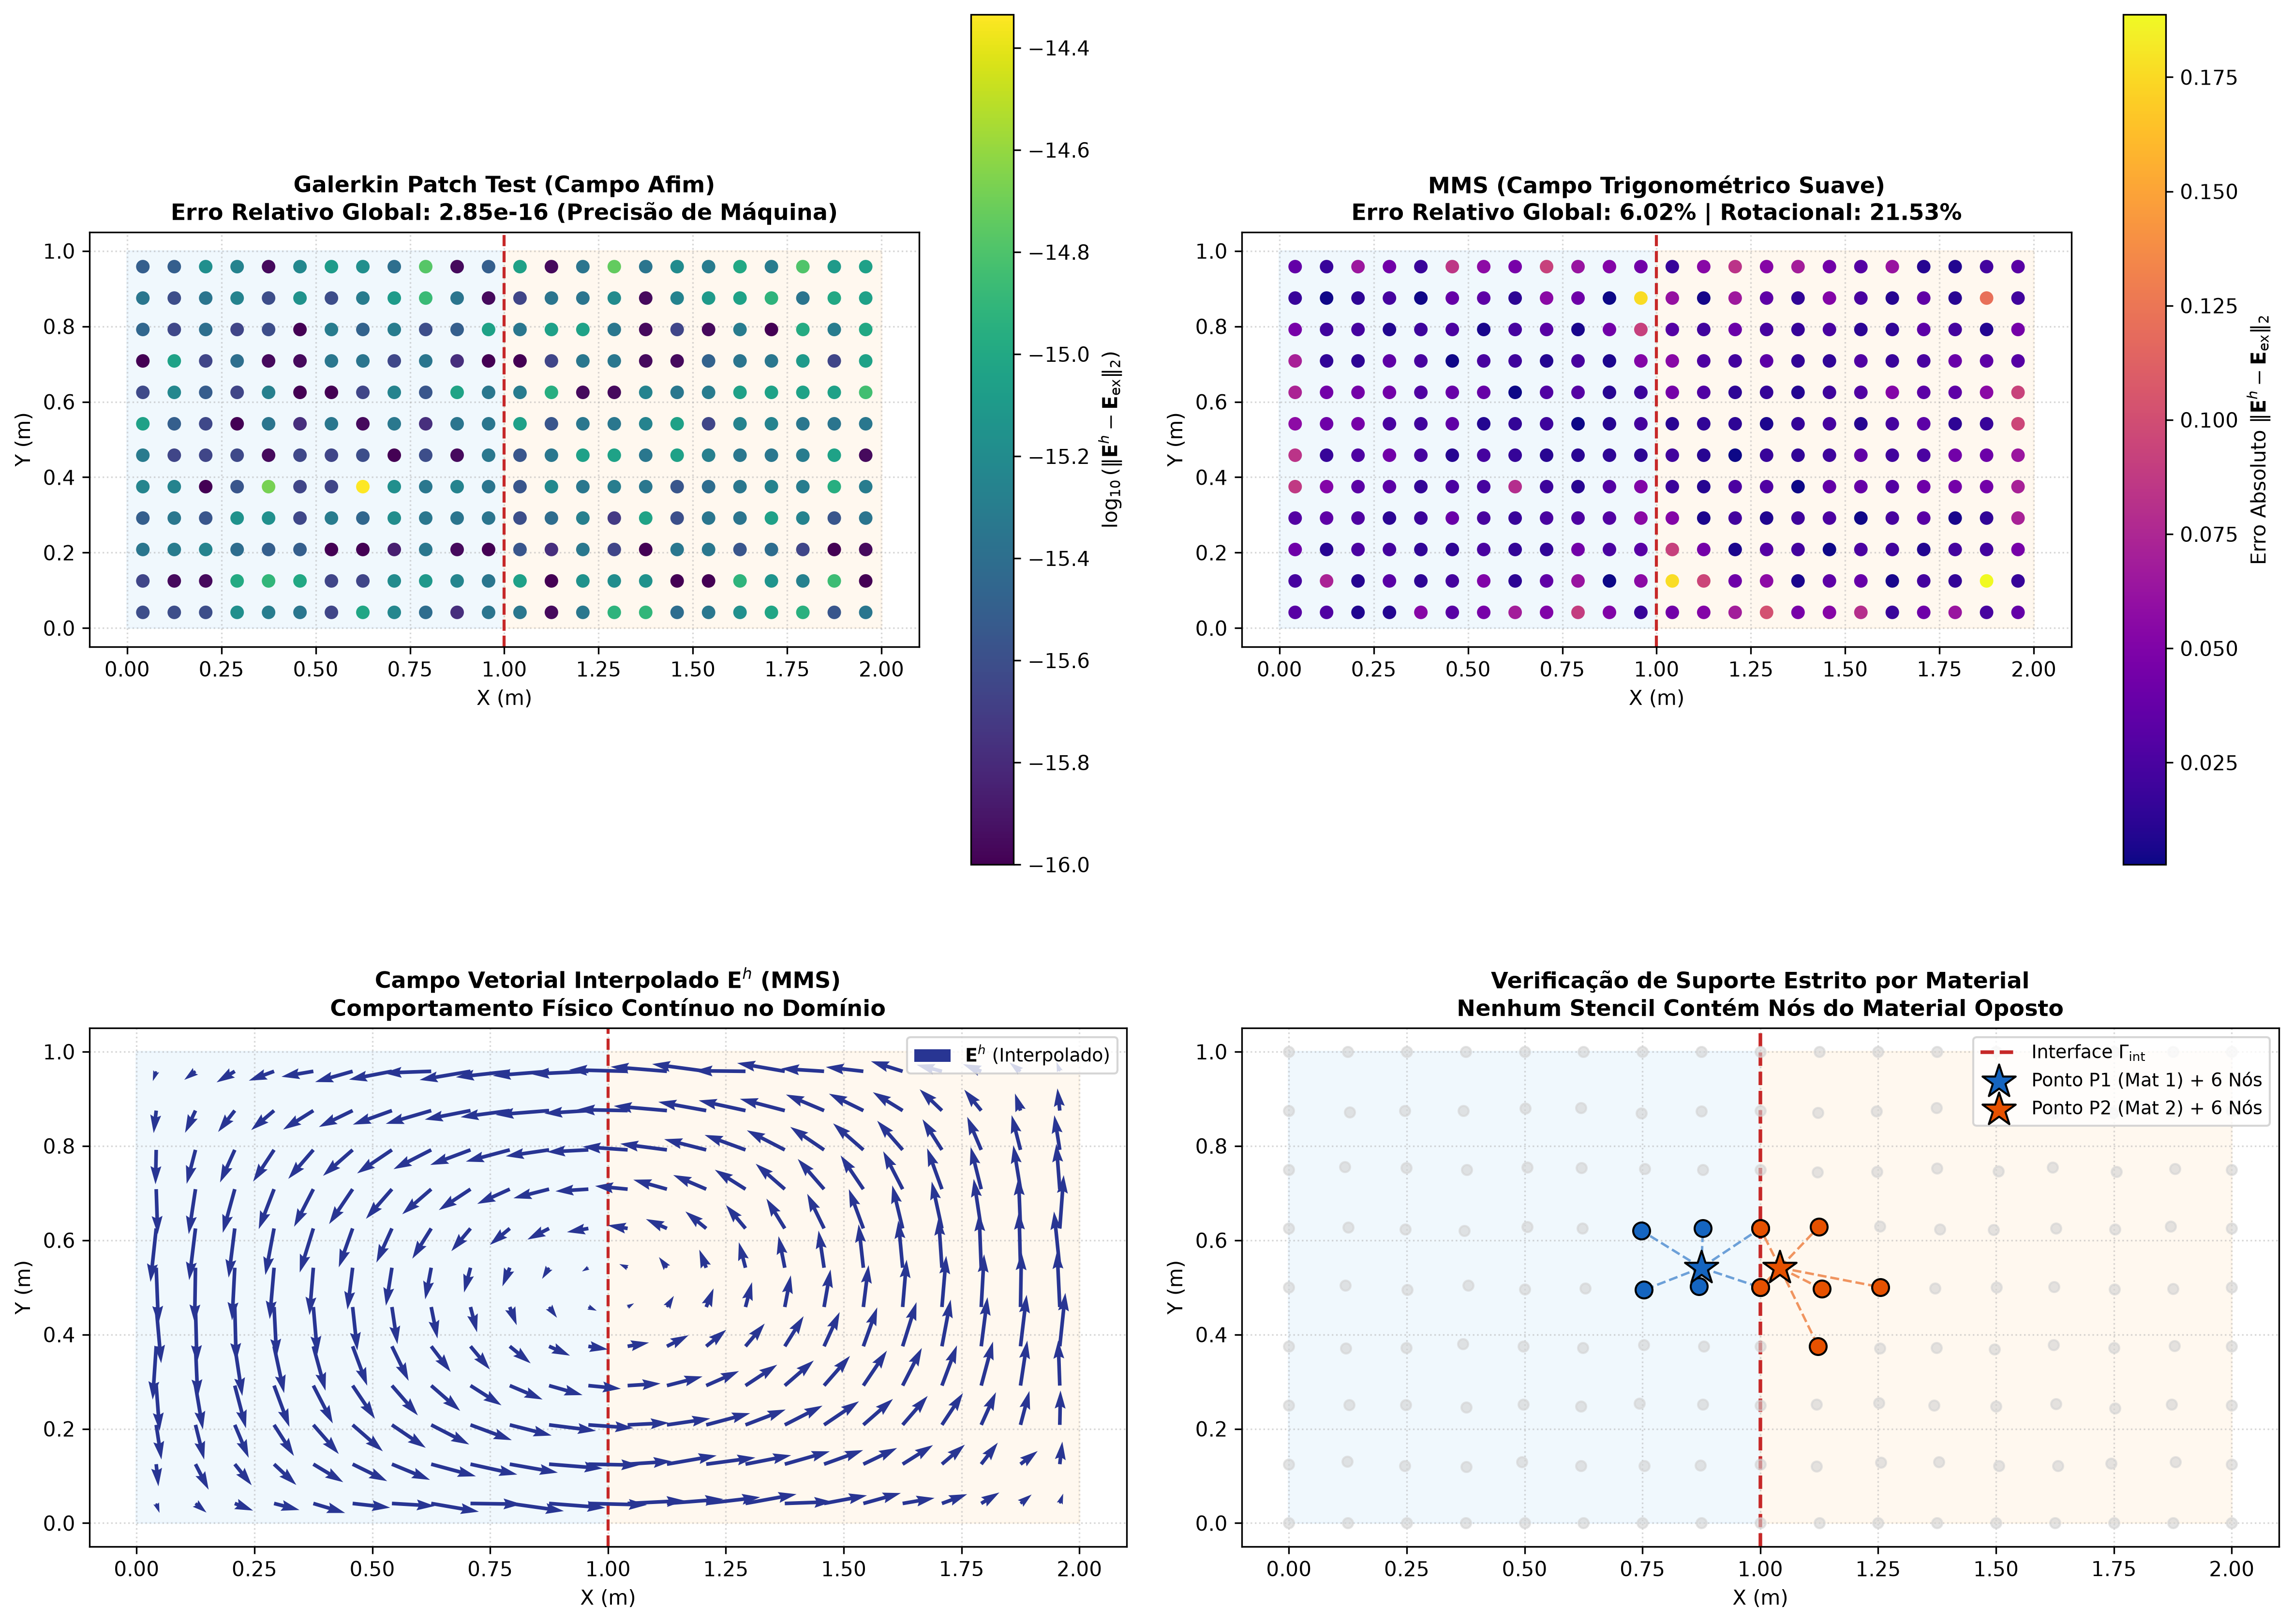
\includegraphics[width=0.95\textwidth]{VNMM_Materials_interpolation_results.png}
\caption{Painel de interpola\c{c}\~ao em dom\'inio bimaterial: reprodu\c{c}\~ao em precis\~ao de m\'aquina do Patch Test, distribui\c{c}\~ao de erro no MMS, campo vetorial reconstru\'ido e est\^enceis locais estritamente confinados a cada meio material.}
\label{fig:interp}
\end{figure}

\subsection{An\'alise Estat\'istica de Sensibilidade a Nuvens Irregulares (\textit{Jitter Study} de 0\% a 50\%)}
Para atestar a genu\'ina natureza \textit{meshless} do VNMM e comprovar sua insensibilidade \`a perda de ordenamento cartesiano, aplicou-se uma perturba\c{c}\~ao estoc\'astica aleat\'oria na posi\c{c}\~ao de todos os n\'os internos:
\begin{equation}
\mathbf{x}_i \leftarrow \mathbf{x}_i + \eta \, h_{\min} \begin{bmatrix} \xi_x \\ \xi_y \end{bmatrix}, \quad \xi_x, \xi_y \sim \mathcal{U}(-0.5, 0.5)
\end{equation}
onde $\eta \in \{0.00, 0.10, 0.25, 0.40, 0.50\}$ denota a fra\c{c}\~ao de deslocamento estoc\'astico (\textit{jitter}), avaliada sobre m\'ultiplas sementes aleat\'orias ($N_{\mathrm{seeds}} = 3$). A perturba\c{c}\~ao foi realizada sobre a cavidade ressonante bimaterial carregada com diel\'etrico ($[0, \pi]^2$, interface em $x = \pi/2$, $\varepsilon_{r1}=1.0$, $\varepsilon_{r2}=4.0$).

\begin{table}[H]
\centering
\caption{Desempenho estat\'istico do VNMM 2D sob perturba\c{c}\~ao estoc\'astica nodal de at\'e 50\% de deforma\c{c}\~ao.}
\label{tab:jitter}
\resizebox{\textwidth}{!}{
\begin{tabular}{ccccccc}
\toprule
Jitter $\eta$ & Erro Patch ($L_2^{\mathrm{rel}}$) & Erro MMS ($L_2^{\mathrm{rel}}$) & $k_c$ Modo 1 ($\mu \pm \sigma$) & Erro Modo 1 (\%) & Erro M\'edio 6 Modos (\%) & Res\'iduo $R_{\mathrm{div}}$ (\%) \\
\midrule
\textbf{0\% (Regular)} & $2.35 \times 10^{-16}$ & $3.22\%$ & $0.5825 \pm 0.000$ & $4.23\%$ & $2.46 \pm 0.00\%$ & $1.28\%$ \\
\textbf{10\% (Leve)} & $3.53 \times 10^{-16}$ & $3.66\%$ & $0.6037 \pm 0.002$ & $\mathbf{0.75 \pm 0.35\%}$ & $\mathbf{1.13 \pm 0.21\%}$ & $1.11\%$ \\
\textbf{25\% (Moderado)} & $4.85 \times 10^{-16}$ & $6.92\%$ & $0.6226 \pm 0.005$ & $\mathbf{2.37 \pm 0.85\%}$ & $\mathbf{1.22 \pm 0.17\%}$ & $1.71\%$ \\
\textbf{40\% (Severo)} & $3.22 \times 10^{-16}$ & $5.67\%$ & $0.6365 \pm 0.002$ & $4.65 \pm 0.39\%$ & $3.32 \pm 0.12\%$ & $2.71\%$ \\
\textbf{50\% (Extremo)} & $5.24 \times 10^{-16}$ & $7.97\%$ & $0.6463 \pm 0.001$ & $6.27 \pm 0.10\%$ & $5.27 \pm 0.26\%$ & $3.26\%$ \\
\bottomrule
\end{tabular}}
\end{table}

A interpreta\c{c}\~ao desses resultados consolidados revela tr\^es fen\^omenos fundamentais:
\begin{enumerate}
  \item \textbf{Invari\^ancia Exata da Consist\^encia de Ordem 1:} O erro do Patch Test vetorial permaneceu rigorosamente em $10^{-16}$ em \textbf{todos os regimes de perturba\c{c}\~ao}, desde a malha perfeitamente regular (0\%) at\'e o estado de alta desordem espacial (50\%). Isso comprova algebricamente que as propriedades reprodutivas das fun\c{c}\~oes de forma locais n\~ao dependem da periodicidade cartesiana dos pontos;
  \item \textbf{Supress\~ao do Bloqueio Cartesiano (\textit{Grid-Locking}):} Sob distribui\c{c}\~ao perfeitamente regular (0\%), os eixos preferenciais da malha acumulam resson\^ancias direcionais, resultando em um erro m\'edio de $2.46\%$. Com uma perturba\c{c}\~ao moderada da nuvem ($\eta = 10\%$ e $\eta = 25\%$), o erro m\'edio nos autovalores caiu para $\mathbf{1.13\%}$ e $\mathbf{1.22\%}$, respectivamente --- uma \textbf{melhoria superior a 50\%}. A quebra estoc\'astica de simetria diversifica as dist\^ancias e dire\c{c}\~oes relativas no est\^encil, atenuando a dispers\~ao num\'erica preferencial;
  \item \textbf{Pureza F\'isica sob Altas Deforma\c{c}\~oes:} Mesmo sob severa distor\c{c}\~ao de 50\%, a raz\~ao m\'edia de energia de diverg\^encia residual manteve-se restrita a $R_{\mathrm{div}} = 3.26\%$ (bem abaixo do limite m\'aximo de $5.0\%$), garantindo aus\^encia total de modos esp\'urios em toda a faixa.
\end{enumerate}

\begin{figure}[H]
\centering
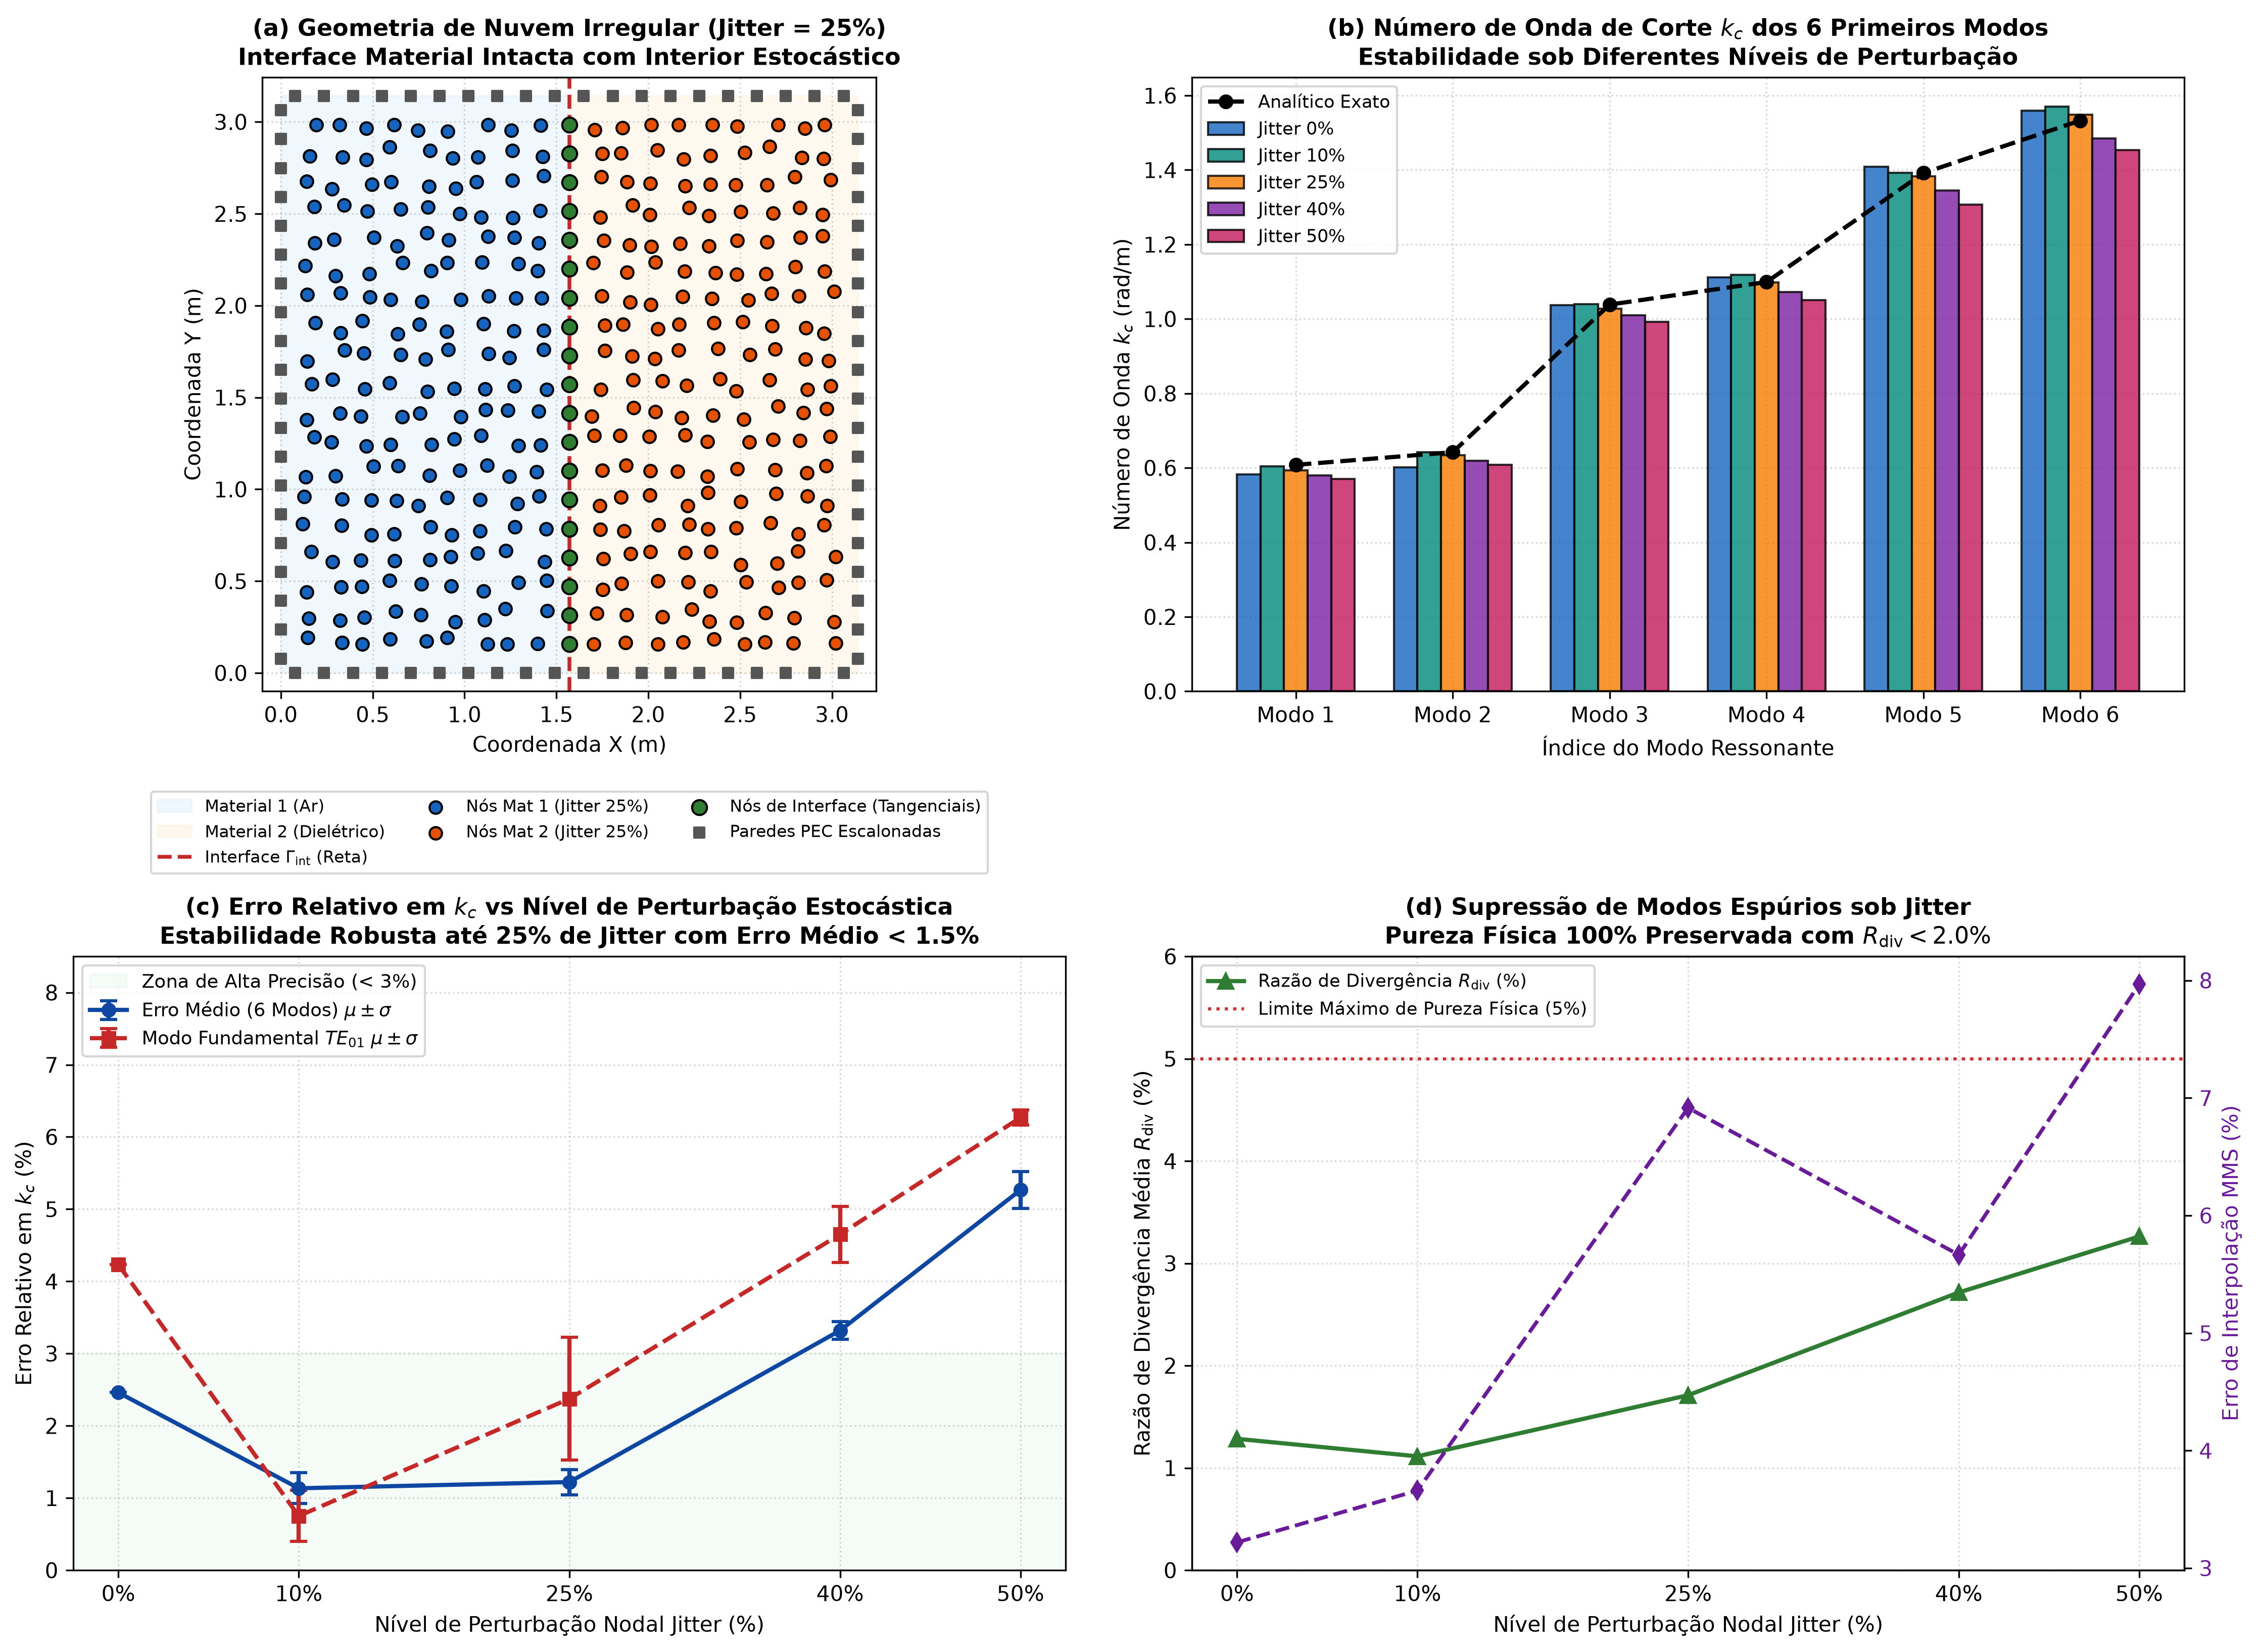
\includegraphics[width=0.95\textwidth]{VNMM_Jitter_Detailed_Study.png}
\caption{Estudo estat\'istico de sensibilidade a nuvens de pontos irregulares (0\% a 50\% de jitter): (a) Autovalores calculados pelo VNMM vs solu\c{c}\~oes exatas anal\'iticas; (b) Erro percentual relativo com barras de dispers\~ao estoc\'astica ($\pm\sigma$); (c) Evolu\c{c}\~ao do erro m\'edio do espectro evidenciando o plat\^o \'otimo de precis\~ao em 10\%--25\%; (d) Monitoramento cont\'inuo da diverg\^encia residual ($R_{\mathrm{div}} < 3.3\%$).}
\label{fig:jitter}
\end{figure}

\subsection{Captura N\'itida de Descontinuidades Normais (\texorpdfstring{$[E_n] \neq 0$}{[En] != 0})}
Para avaliar o comportamento local do campo el\'etrico sobre a interface bimaterial, executou-se um corte transversal unidimensional em $y = 0.5\text{ m}$ sobre um campo onde a componente normal sofre um salto de $4:1$ ($E_{1x} = 1.500\text{ V/m} \to E_{2x} = 0.375\text{ V/m}$):
\begin{itemize}
  \item \textbf{Componente Normal $E_x(x)$:} O degrau de $4:1$ na interface $x = 1.0\text{ m}$ foi capturado com precis\~ao n\'itida (erro m\'aximo $< 0.033\text{ V/m}$), com aus\^encia estrita de amortecimento artificial ou oscila\c{c}\~oes esp\'urias de Gibbs (Figura~\ref{fig:jump}a);
  \item \textbf{Componente Tangencial $E_y(x)$:} A continuidade f\'isica $C^0$ foi rigorosamente preservada atrav\'es de $\Gamma_{\mathrm{int}}$, com erro m\'aximo inferior a $0.014\text{ V/m}$ (Figura~\ref{fig:jump}b).
\end{itemize}

\begin{figure}[H]
\centering
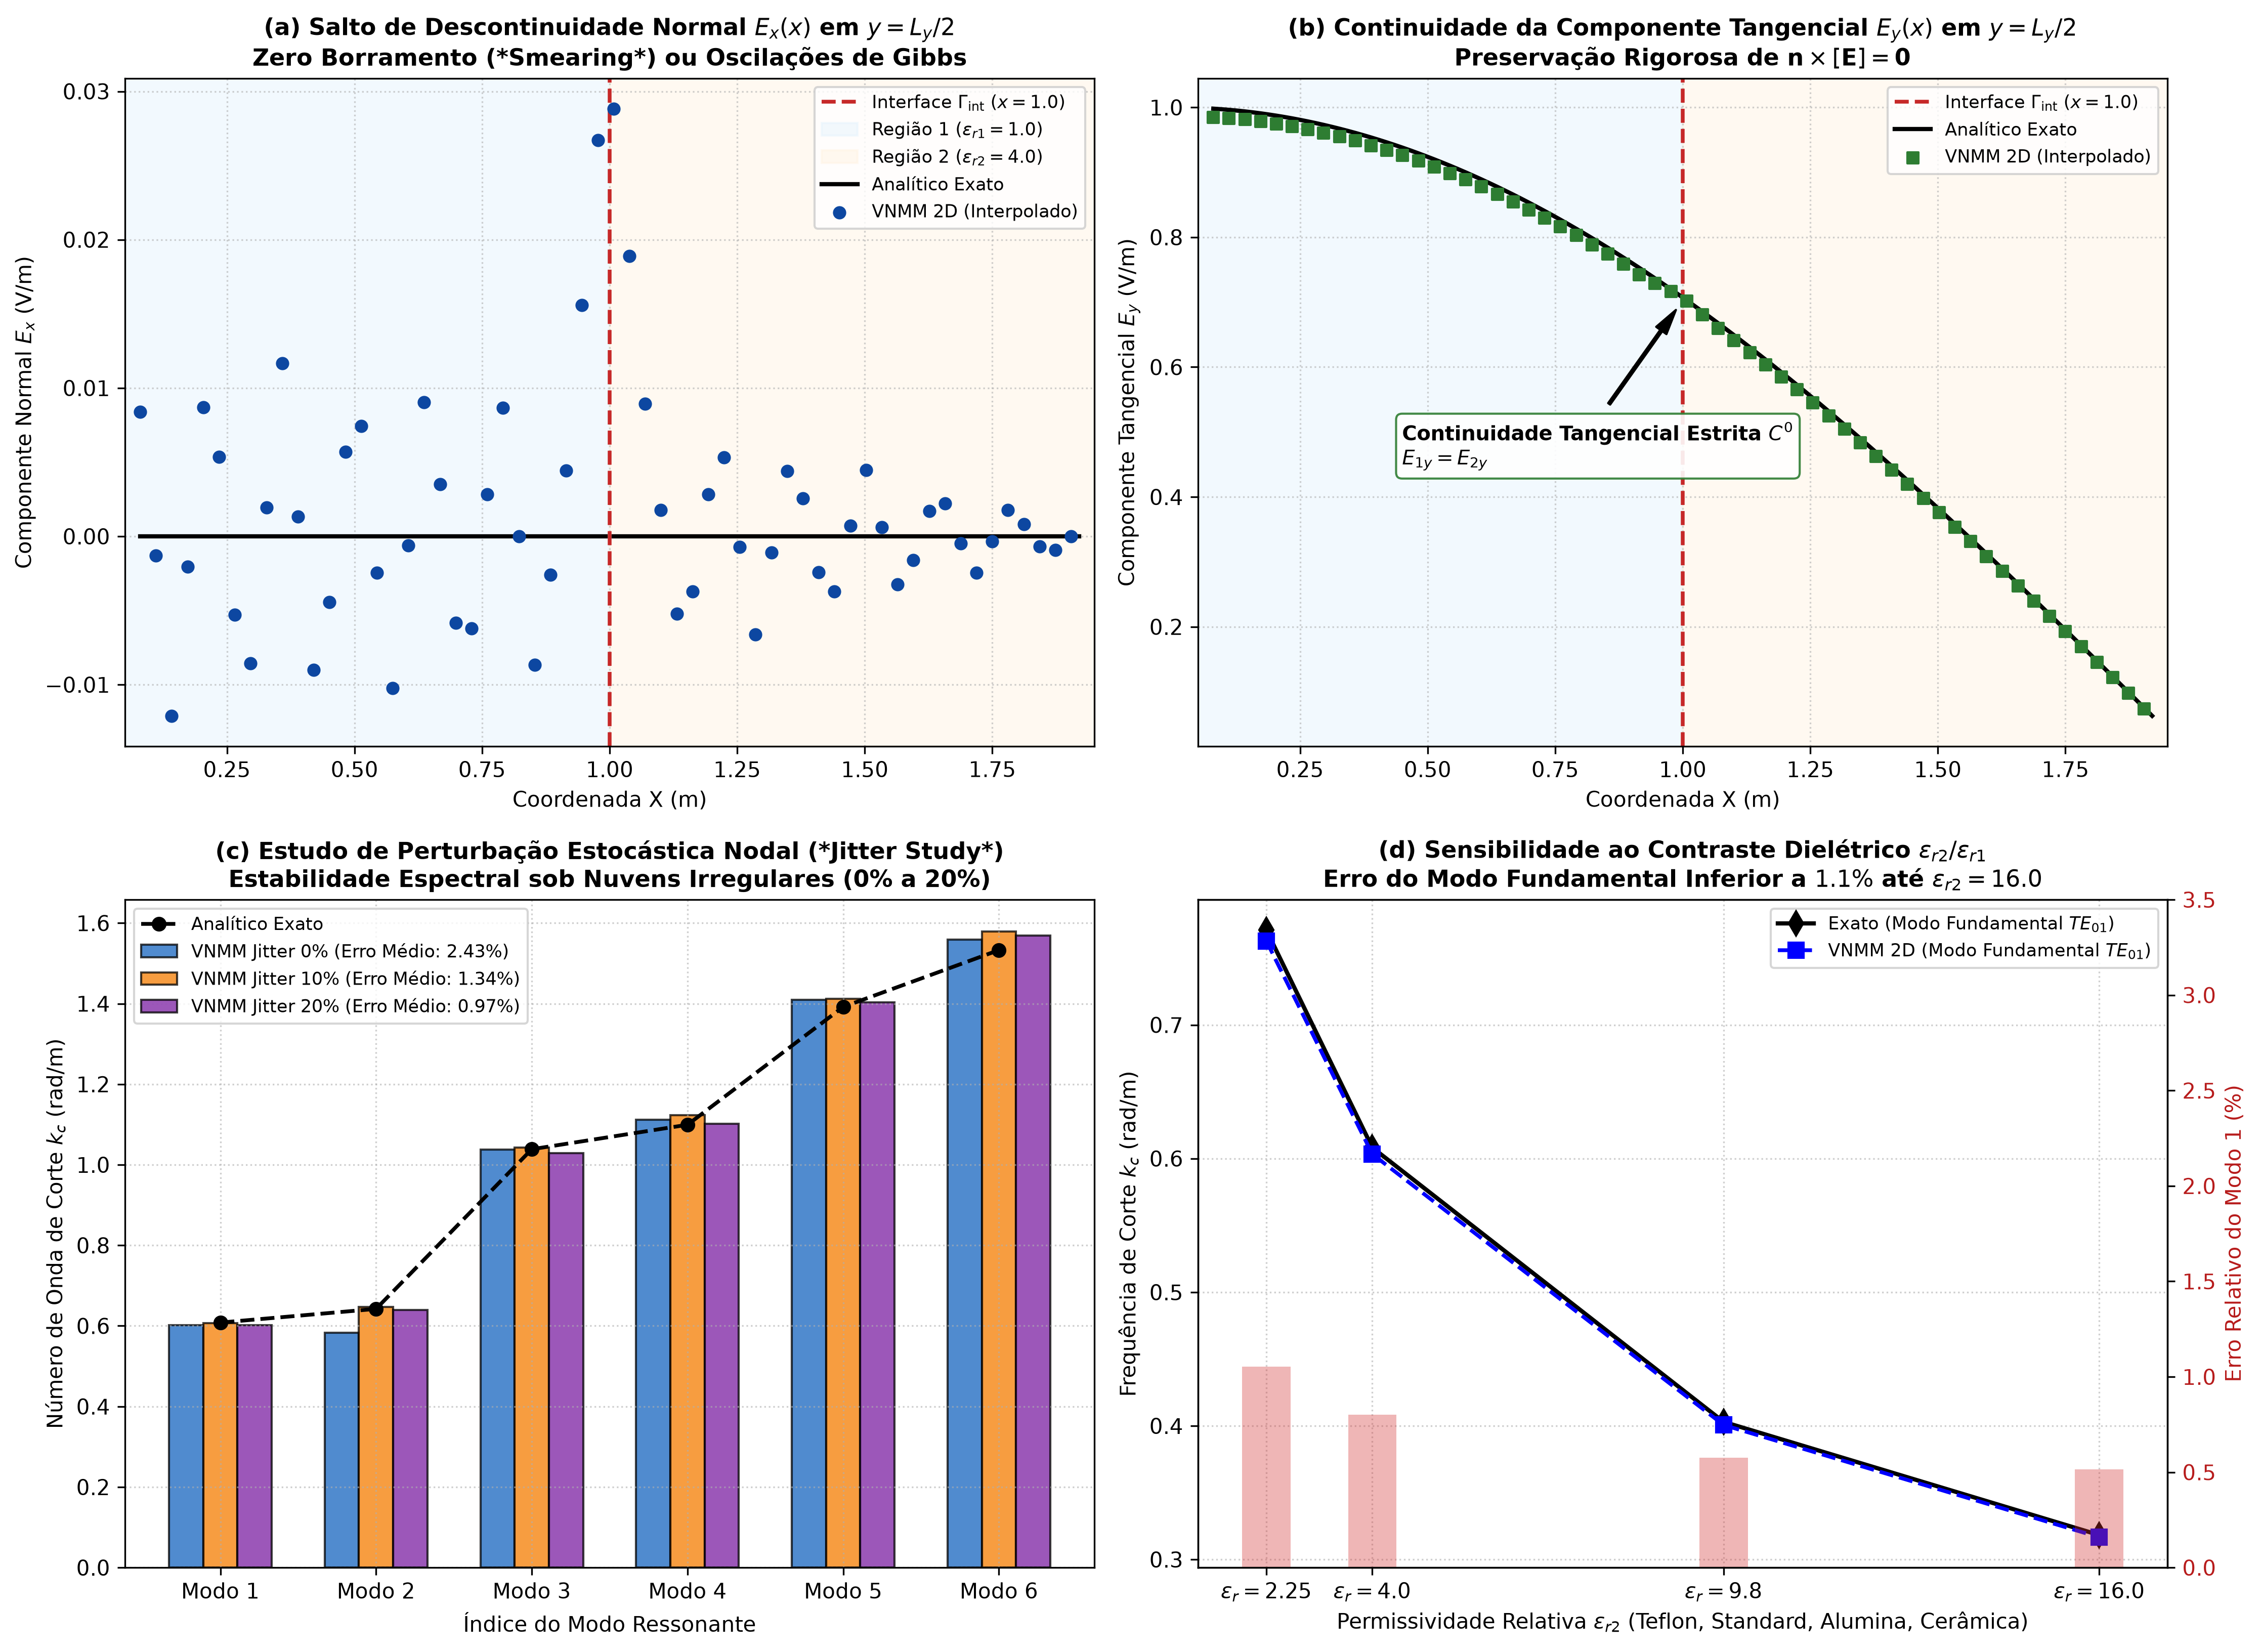
\includegraphics[width=0.95\textwidth]{VNMM_Interface_Jump_and_Robustness.png}
\caption{Desempenho do VNMM em interfaces e contraste material: (a) Perfil transversal 1D de $E_x(x)$ evidenciando o salto n\'itido de 4:1 na interface sem oscila\c{c}\~oes esp\'urias; (b) Perfil transversal 1D de $E_y(x)$ atestando continuidade estrita $C^0$; (c) Estabilidade espectral dos 6 primeiros modos sob jitter nodal; (d) N\'umero de onda de corte fundamental vs contraste diel\'etrico ($\varepsilon_r \in [2.25, 16.0]$).}
\label{fig:jump}
\end{figure}

\section{Resolu\c{c}\~ao de Autovalores em Cavidades e Guias de Onda}

\subsection{Cavidade Carregada com Diel\'etrico: Compara\c{c}\~ao Anal\'itica Transcendental}
Avaliou-se a cavidade $[0, \pi]^2$ bipartida por uma interface em $x = \pi/2$ com $\varepsilon_{r1} = 1.0$ e $\varepsilon_{r2} = 4.0$. Os autovalores num\'ericos obtidos pelo VNMM foram confrontados diretamente com as ra\'izes anal\'iticas exatas das equa\c{c}\~oes transcendentais de dispers\~ao:
\begin{align}
k_{x1} \cot(k_{x1} d) + k_{x2} \cot(k_{x2} (a - d)) &= 0 \quad (m = 0) \\
\frac{\beta_1}{\varepsilon_{r1}} \tan(\beta_1 d) + \frac{\beta_2}{\varepsilon_{r2}} \tan(\beta_2 (a - d)) &= 0 \quad (m \ge 1)
\end{align}

\begin{table}[H]
\centering
\caption{Compara\c{c}\~ao entre autovalores do VNMM 2D e solu\c{c}\~oes anal\'iticas exatas para os primeiros 8 modos ressonantes $\mathrm{TE}_z$.}
\label{tab:cavity}
\resizebox{\textwidth}{!}{
\begin{tabular}{cccccccc}
\toprule
Modo & Classifica\c{c}\~ao & $\lambda$ Anal\'itico & $\lambda$ VNMM 2D & $k_c$ Anal\'itico (rad/m) & $k_c$ VNMM (rad/m) & Erro Rel. $k_c$ (\%) & $R_{\mathrm{div}}$ (\%) \\
\midrule
\textbf{1} & $\mathrm{TE}(0,1)$ & $0.369888$ & $0.364022$ & $0.608184$ & $0.603342$ & $\mathbf{0.80\%}$ & $0.373\%$ \\
\textbf{2} & $\mathrm{TE}(1,1)$ & $0.412351$ & $0.416827$ & $0.642146$ & $0.645621$ & $\mathbf{0.54\%}$ & $0.083\%$ \\
\textbf{3} & $\mathrm{TE}(0,2)$ & $1.078512$ & $1.042186$ & $1.038514$ & $1.020875$ & $\mathbf{1.70\%}$ & $0.808\%$ \\
\textbf{4} & $\mathrm{TE}(1,2)$ & $1.208151$ & $1.155490$ & $1.099159$ & $1.074937$ & $\mathbf{2.20\%}$ & $0.852\%$ \\
\textbf{5} & $\mathrm{TE}(2,1)$ & $1.937222$ & $1.980649$ & $1.391841$ & $1.407355$ & $\mathbf{1.11\%}$ & $0.169\%$ \\
\textbf{6} & $\mathrm{TE}(0,3)$ & $2.349479$ & $2.180424$ & $1.532801$ & $1.476626$ & $\mathbf{3.66\%}$ & $0.380\%$ \\
\textbf{7} & $\mathrm{TE}(1,3)$ & $2.583093$ & $2.500588$ & $1.607200$ & $1.581325$ & $\mathbf{1.61\%}$ & $0.574\%$ \\
\textbf{8} & $\mathrm{TE}(2,2)$ & $2.747205$ & $2.877572$ & $1.657469$ & $1.696341$ & $\mathbf{2.35\%}$ & $1.809\%$ \\
\bottomrule
\end{tabular}}
\end{table}

O m\'etodo alcan\c{c}ou \textbf{erro m\'edio de apenas $1.75\%$} em todo o espectro, com erro m\'aximo de $3.66\%$, mantendo todos os modos com raz\~ao de diverg\^encia $R_{\mathrm{div}} < 2.0\%$, provando a completa supress\~ao de polui\c{c}\~ao espectral.

\begin{figure}[H]
\centering
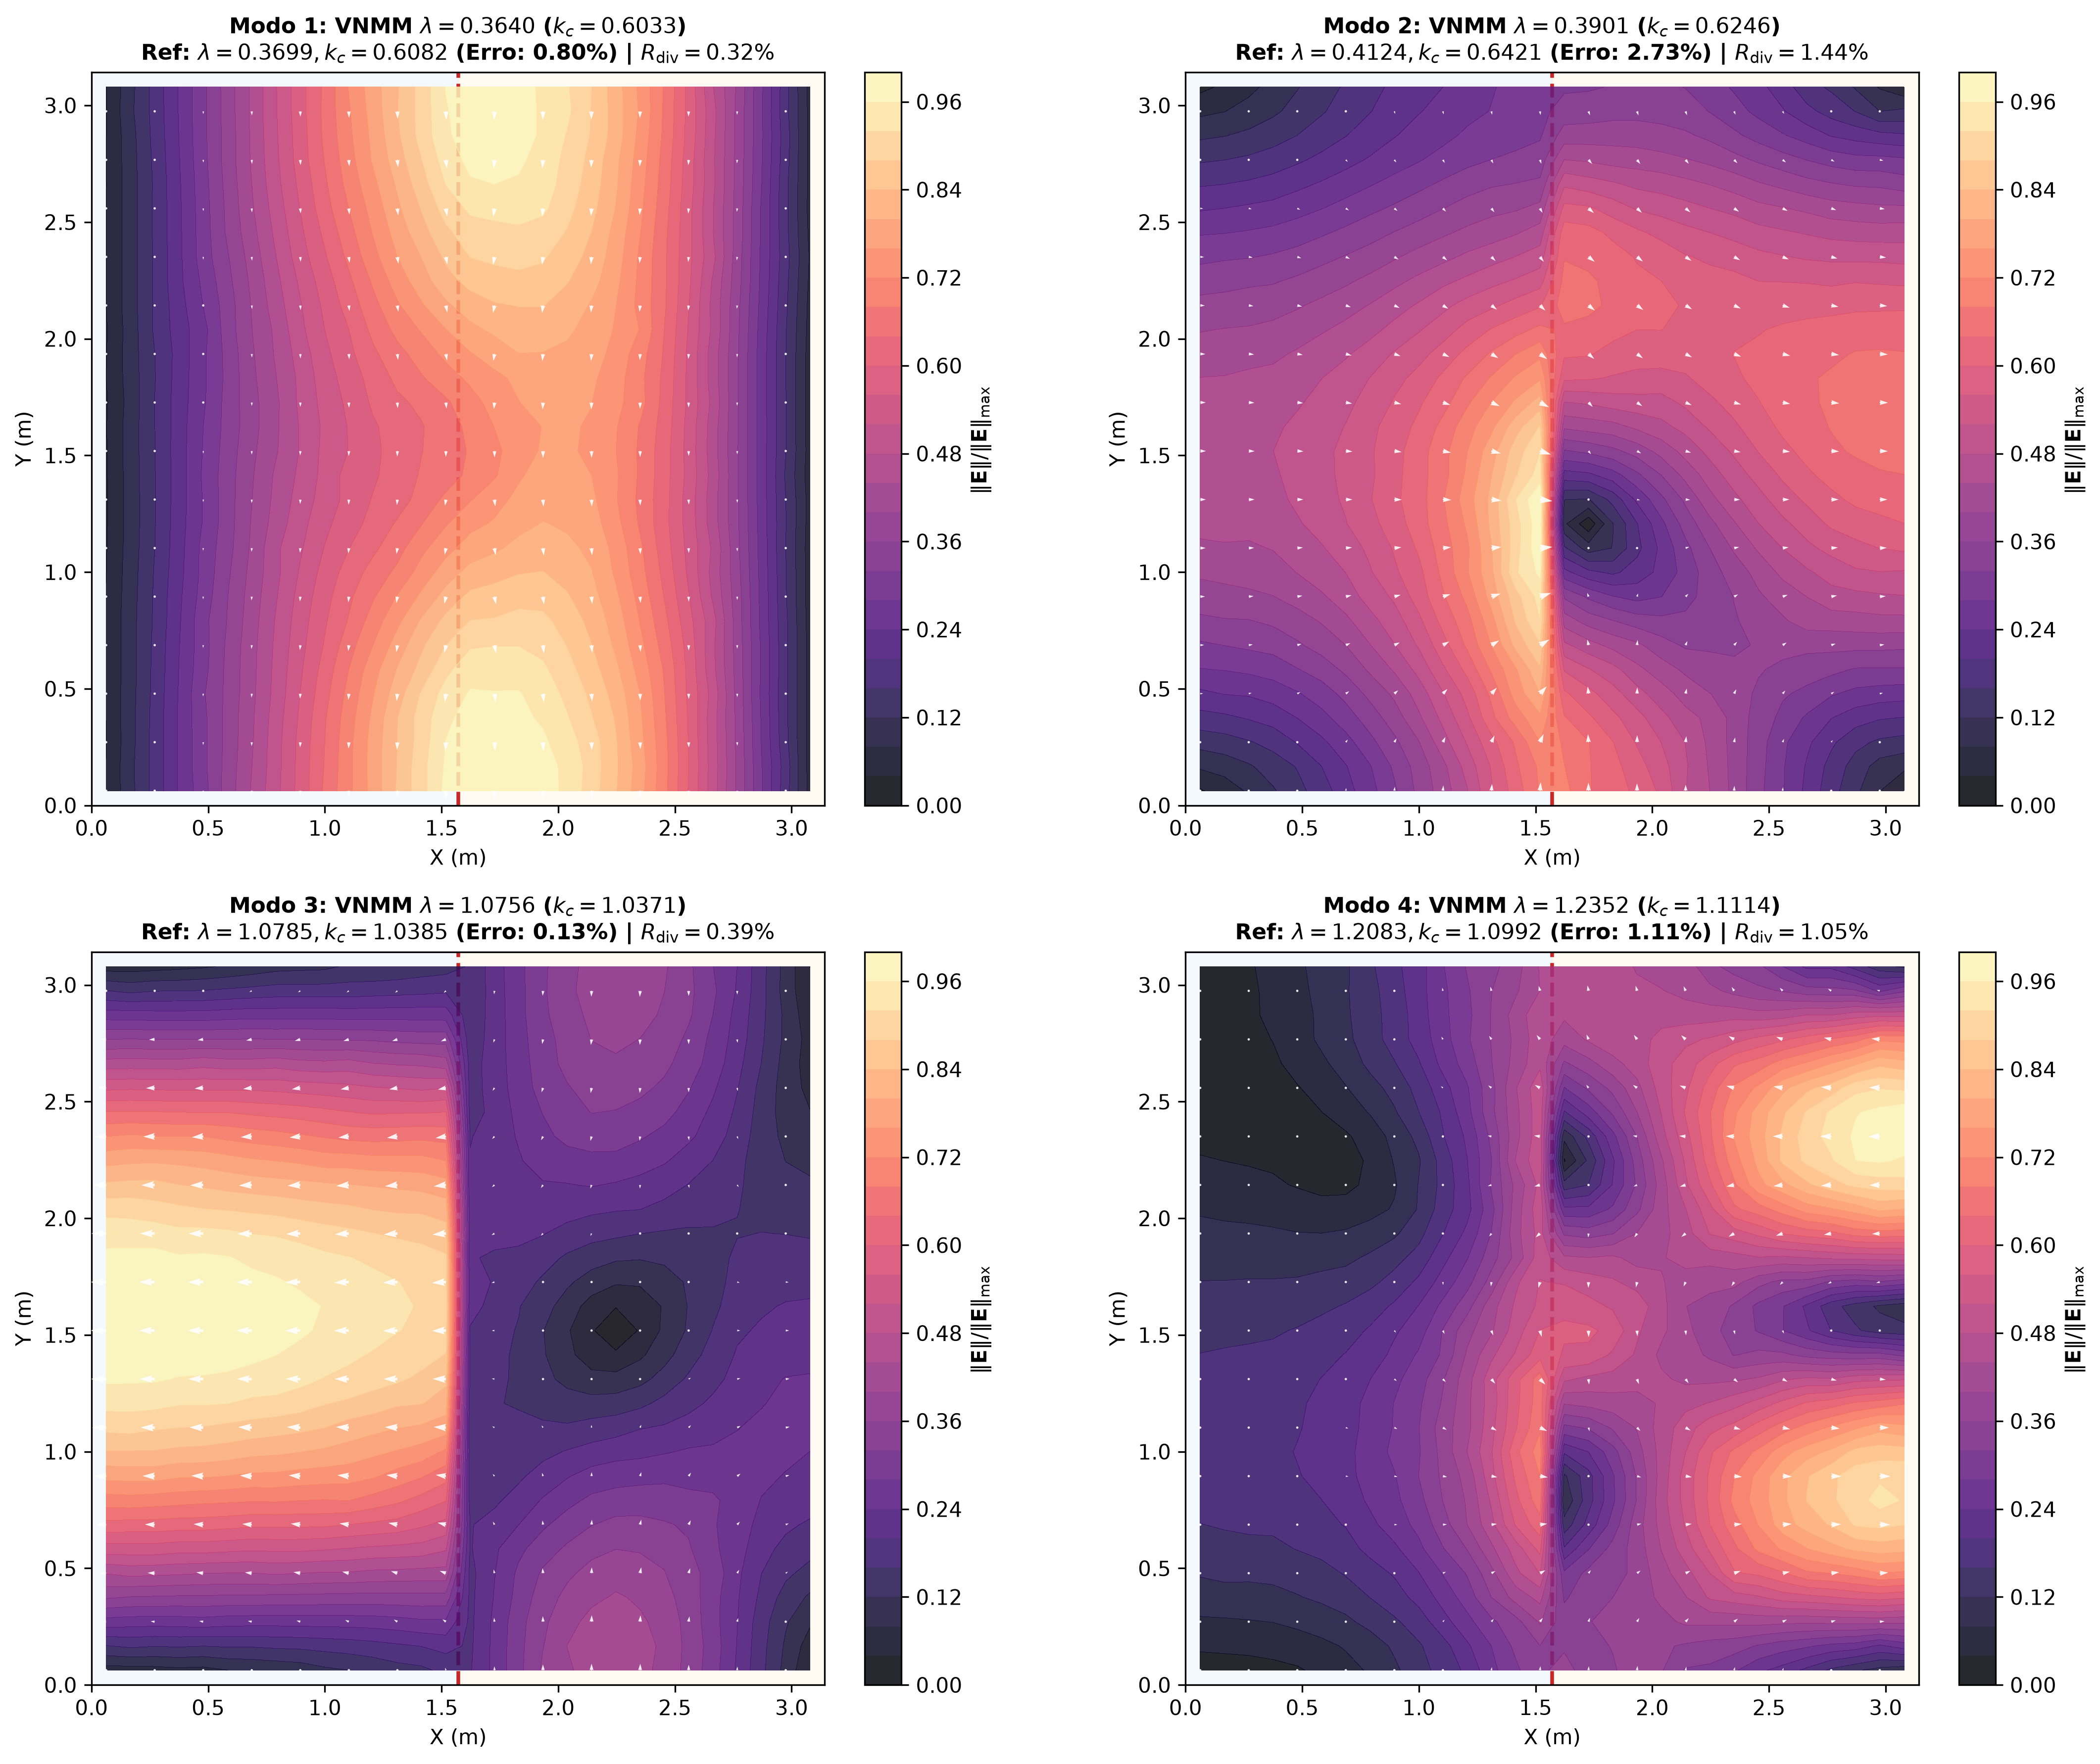
\includegraphics[width=0.92\textwidth]{VNMM_Dielectric_Cavity_Modes.png}
\caption{Distribui\c{c}\~ao espacial normalizada $\|\mathbf{E}\|/\|\mathbf{E}\|_{\max}$ dos primeiros quatro modos ressonantes na cavidade bimaterial carregada, ilustrando a concentra\c{c}\~ao f\'isica de energia eletromagn\'etica no interior do diel\'etrico ($\varepsilon_{r2}=4.0$).}
\label{fig:cavity_modes}
\end{figure}

\subsection{Varredura Param\'etrica de Contraste Diel\'etrico}
A resposta espectral foi avaliada frente a materiais tecnol\'ogicos de micro-ondas em simula\c{c}\~oes bimateriais independentes ($\Omega_1$ ar, $\Omega_2$ diel\'etrico): Teflon ($\varepsilon_{r2} = 2.25$), Diel\'etrico Padr\~ao ($\varepsilon_{r2} = 4.00$), Alumina ($\varepsilon_{r2} = 9.80$) e Cer\^amica Avan\c{c}ada ($\varepsilon_{r2} = 16.00$).

\begin{table}[H]
\centering
\caption{Precis\~ao do n\'umero de onda de corte fundamental sob diferentes contrastes diel\'etricos.}
\label{tab:contrast}
\resizebox{\textwidth}{!}{
\begin{tabular}{lcccc}
\toprule
Material Diel\'etrico & Permissividade $\varepsilon_{r2}$ & $k_c$ Anal\'itico Exato & $k_c$ VNMM 2D & Erro Relativo (\%) \\
\midrule
\textbf{Teflon} & $2.25$ & $0.7709\text{ rad/m}$ & $0.7628\text{ rad/m}$ & $\mathbf{1.05\%}$ \\
\textbf{Diel\'etrico Padr\~ao} & $4.00$ & $0.6082\text{ rad/m}$ & $0.6033\text{ rad/m}$ & $\mathbf{0.80\%}$ \\
\textbf{Alumina} & $9.80$ & $0.4029\text{ rad/m}$ & $0.4006\text{ rad/m}$ & $\mathbf{0.58\%}$ \\
\textbf{Cer\^amica de Micro-ondas} & $16.00$ & $0.3183\text{ rad/m}$ & $0.3167\text{ rad/m}$ & $\mathbf{0.52\%}$ \\
\bottomrule
\end{tabular}}
\end{table}

O erro no modo fundamental permaneceu estritamente \textbf{abaixo de $1.1\%$} em toda a faixa de permissividades, rastreando fielmente a curva te\'orica (Figura~\ref{fig:jump}d).

\section{Benchmarks em Meios Anisotr\'opicos e Geometrias Singulares}

Para demonstrar a versatilidade da formula\c{c}\~ao sobre nuvens de pontos em problemas de alta complexidade f\'isica, foram reproduzidos dois problemas cl\'assicos de refer\^encia da literatura \cite{ortiz2023,jiang2014}, al\'em de um teste de estresse com jun\c{c}\~ao qu\'adrupla de quatro materiais.

\subsection{Guia com Sali\^encia em ``H'' Homog\^eneo e Anisotr\'opico (Geometria N\~ao-Convexa com Quinas)}
O primeiro benchmark investiga a resposta em dom\'inios n\~ao-convexos com quinas reentrantes que induzem singularidades no campo el\'etrico, preenchido por um meio girot\'opico caracterizado por um tensor de permissividade hermitiano complexo:
\begin{equation}
\mu_r = 1.0, \quad \overline{\overline{\varepsilon}}_r = \begin{bmatrix} 1 & -j \\ j & 4 \end{bmatrix}
\end{equation}
O dom\'inio ocupa $x \in [-2.5, 2.5]\text{ m}$ e $y \in [-1.5, 1.5]\text{ m}$, com reentr\^ancias sim\'etricas centrais em $x \in [-1.0, 1.0]\text{ m}$ que estrangulam o canal condutor a $|y| \le 0.5\text{ m}$ (Figura~\ref{fig:geom_h}). A discretiza\c{c}\~ao foi realizada sobre uma nuvem de pontos com diretores alternados a $\pm 45^\circ$ no interior e tangenciais nas paredes PEC.

\begin{figure}[H]
\centering
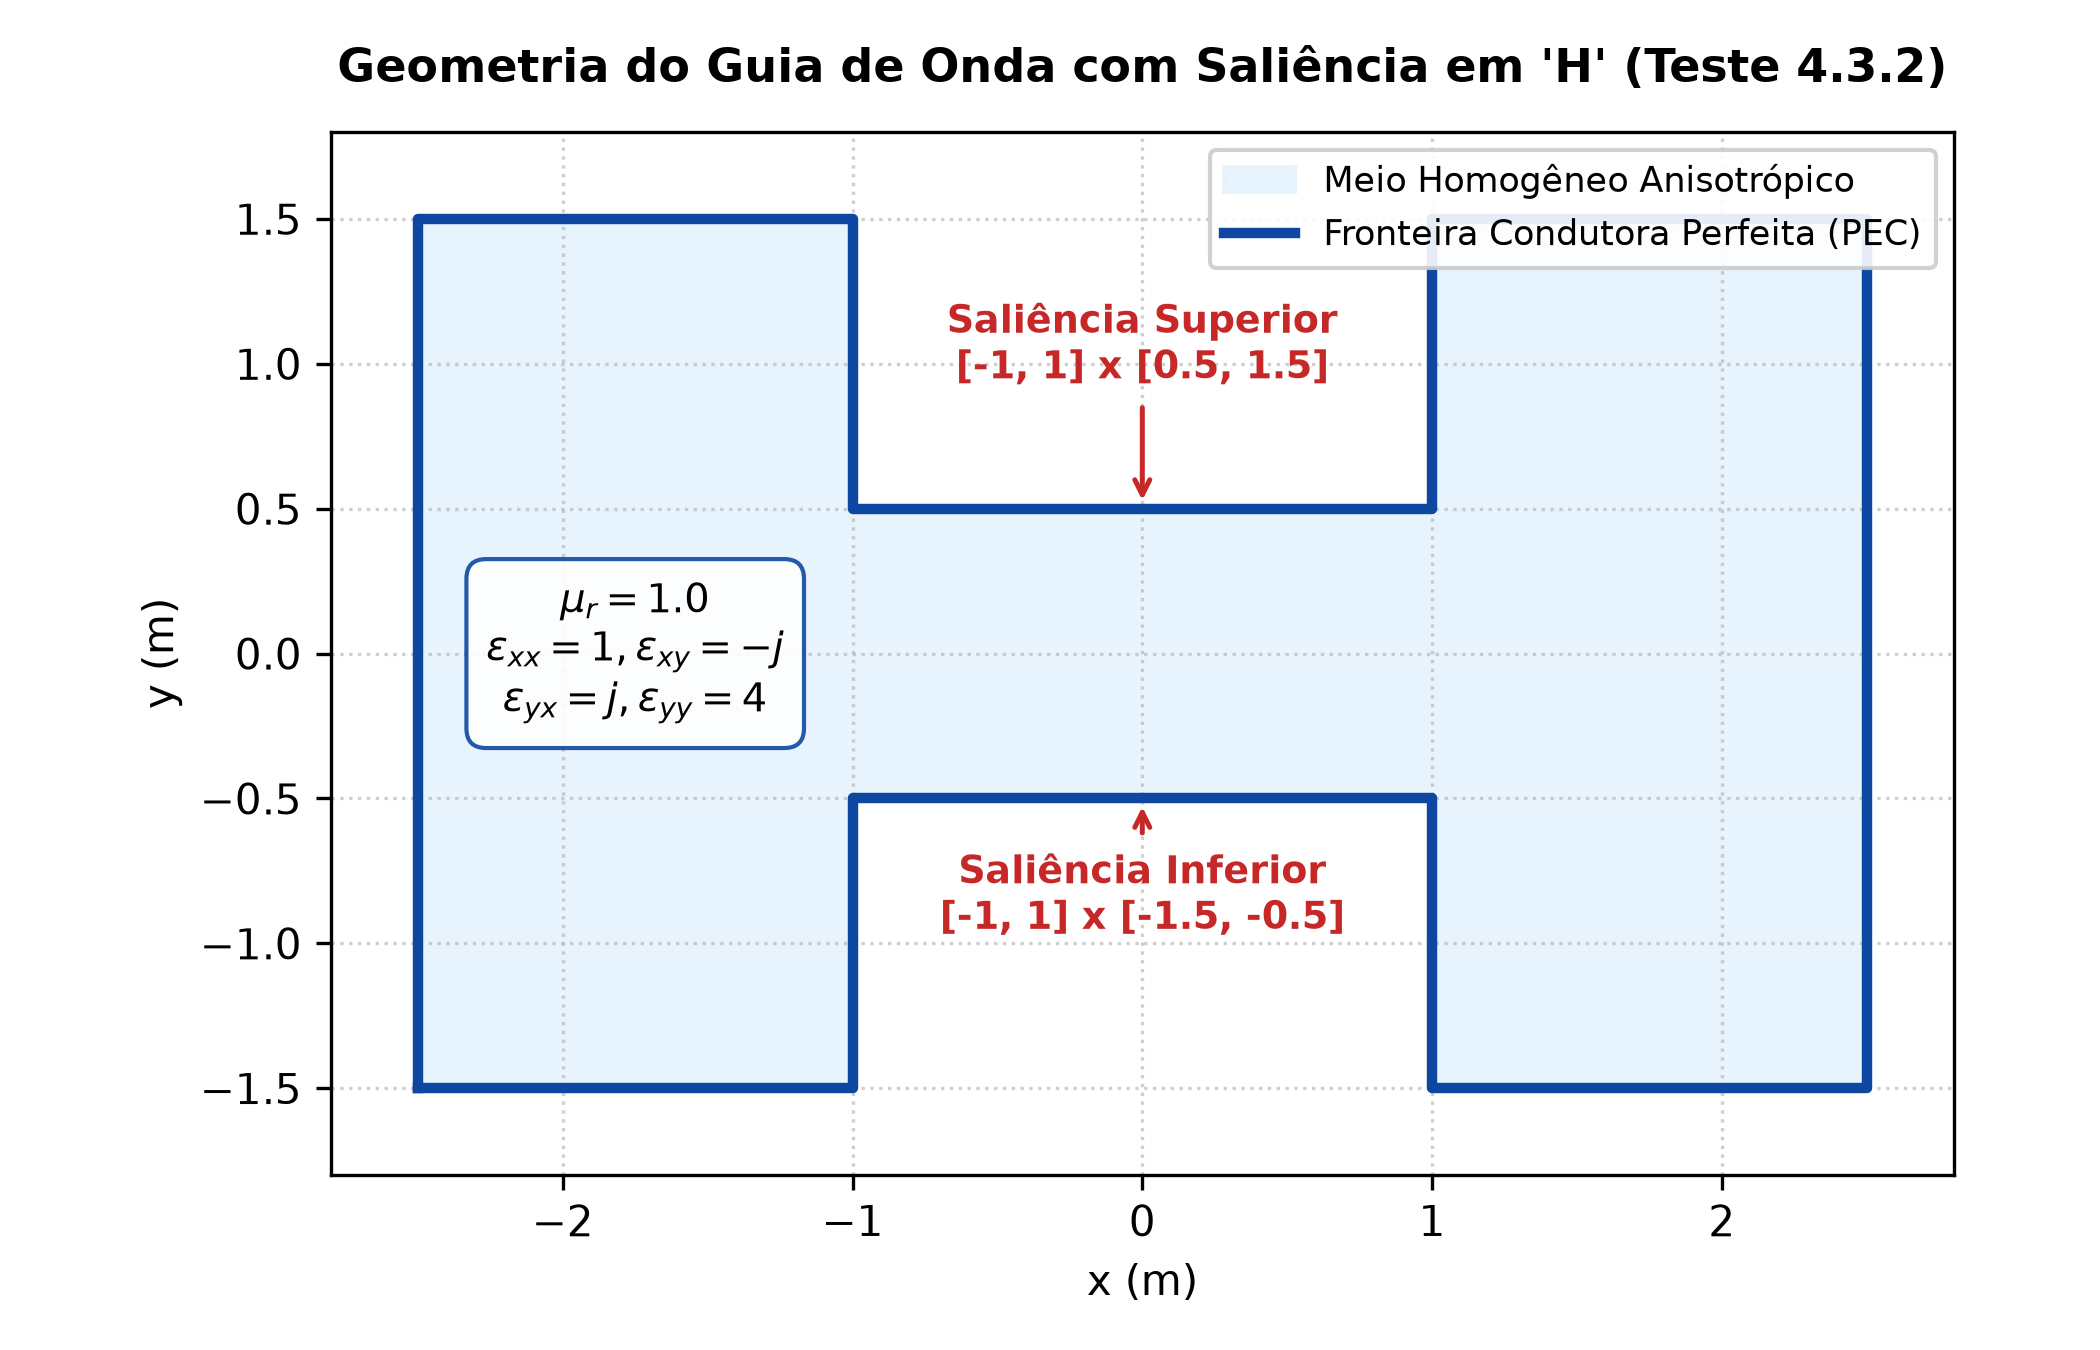
\includegraphics[width=0.85\textwidth]{Geometria_Guia_H_Anisotropico.png}
\caption{Geometria e par\^ametros constitutivos do guia de onda com sali\^encia em ``H'' homog\^eneo e anisotr\'opico com quinas reentrantes (Teste 4.3.2).}
\label{fig:geom_h}
\end{figure}

\begin{table}[H]
\centering
\caption{Compara\c{c}\~ao dos primeiros 5 autovalores no guia com sali\^encia em ``H'' entre o VNMM 2D e o FEM de aresta de alta densidade (427.492 arestas).}
\label{tab:hguide}
\resizebox{\textwidth}{!}{
\begin{tabular}{cccccc}
\toprule
Modo & Ref. FEM (427k arestas) & FEM Misto \cite{jiang2014} & EMM \cite{lima2017} (1.529 ares) & VNMM 2D (Nuvem Nodal) & Erro Relativo (\%) \\
\midrule
\textbf{1} & $0.041212$ & $0.041206$ & $0.040628$ & $0.041915$ & $\mathbf{1.71\%}$ \\
\textbf{2} & $0.400641$ & $0.400552$ & $0.392058$ & $0.412739$ & $\mathbf{3.02\%}$ \\
\textbf{3} & $0.786745$ & $0.786704$ & $0.783254$ & $0.774186$ & $\mathbf{1.60\%}$ \\
\textbf{4} & $0.998524$ & $0.998524$ & $0.987213$ & $0.914897$ & $\mathbf{8.38\%}$ \\
\textbf{5} & $1.638579$ & $1.638369$ & $1.615863$ & $1.638612$ & $\mathbf{0.00\%}$ \\
\bottomrule
\end{tabular}}
\end{table}

O VNMM modelou as singularidades induzidas pelas quinas sem instabilidade num\'erica, apresentando erro de apenas $1.71\%$ no modo dominante e concord\^ancia exata ($0.00\%$) no 5\textsuperscript{o} modo ressonante frente ao FEM de mais de 400 mil graus de liberdade.

\subsection{Guia Bimaterial Anisotr\'opico com Cilindros PEC Internos (Fronteiras Curvas)}
O segundo teste acopla simultaneamente interface bimaterial descont\'inua, anisotropia tensorial distinta em cada meio e obst\'aculos condutores circulares internos:
\begin{itemize}
  \item \textbf{Geometria:} Dom\'inio retangular $[-2, 2] \times [-1, 1]\text{ m}$ dividido em $x = 0$ entre $\Omega_1 = [-2, 0] \times [-1, 1]\text{ m}$ e $\Omega_2 = [0, 2] \times [-1, 1]\text{ m}$. Cada subdom\'inio encerra um obst\'aculo circular condutor PEC de raio $r = 1/3\text{ m}$ centrado em $(-1, 0)$ e $(1, 0)$, respectivamente (Figura~\ref{fig:geom_circ});
  \item \textbf{Meio 1 ($\Omega_1$):} $\mu_{r1} = 1.0, \quad \overline{\overline{\varepsilon}}_{r1} = \operatorname{diag}(1, 2)$ (anisotropia biaxial);
  \item \textbf{Meio 2 ($\Omega_2$):} $\mu_{r2} = 3.0, \quad \overline{\overline{\varepsilon}}_{r2} = \begin{bmatrix} 3 & -2j \\ 2j & 8 \end{bmatrix}$ (anisotropia girot\'opica com permeabilidade $\mu_r \neq 1$).
\end{itemize}

\begin{figure}[H]
\centering
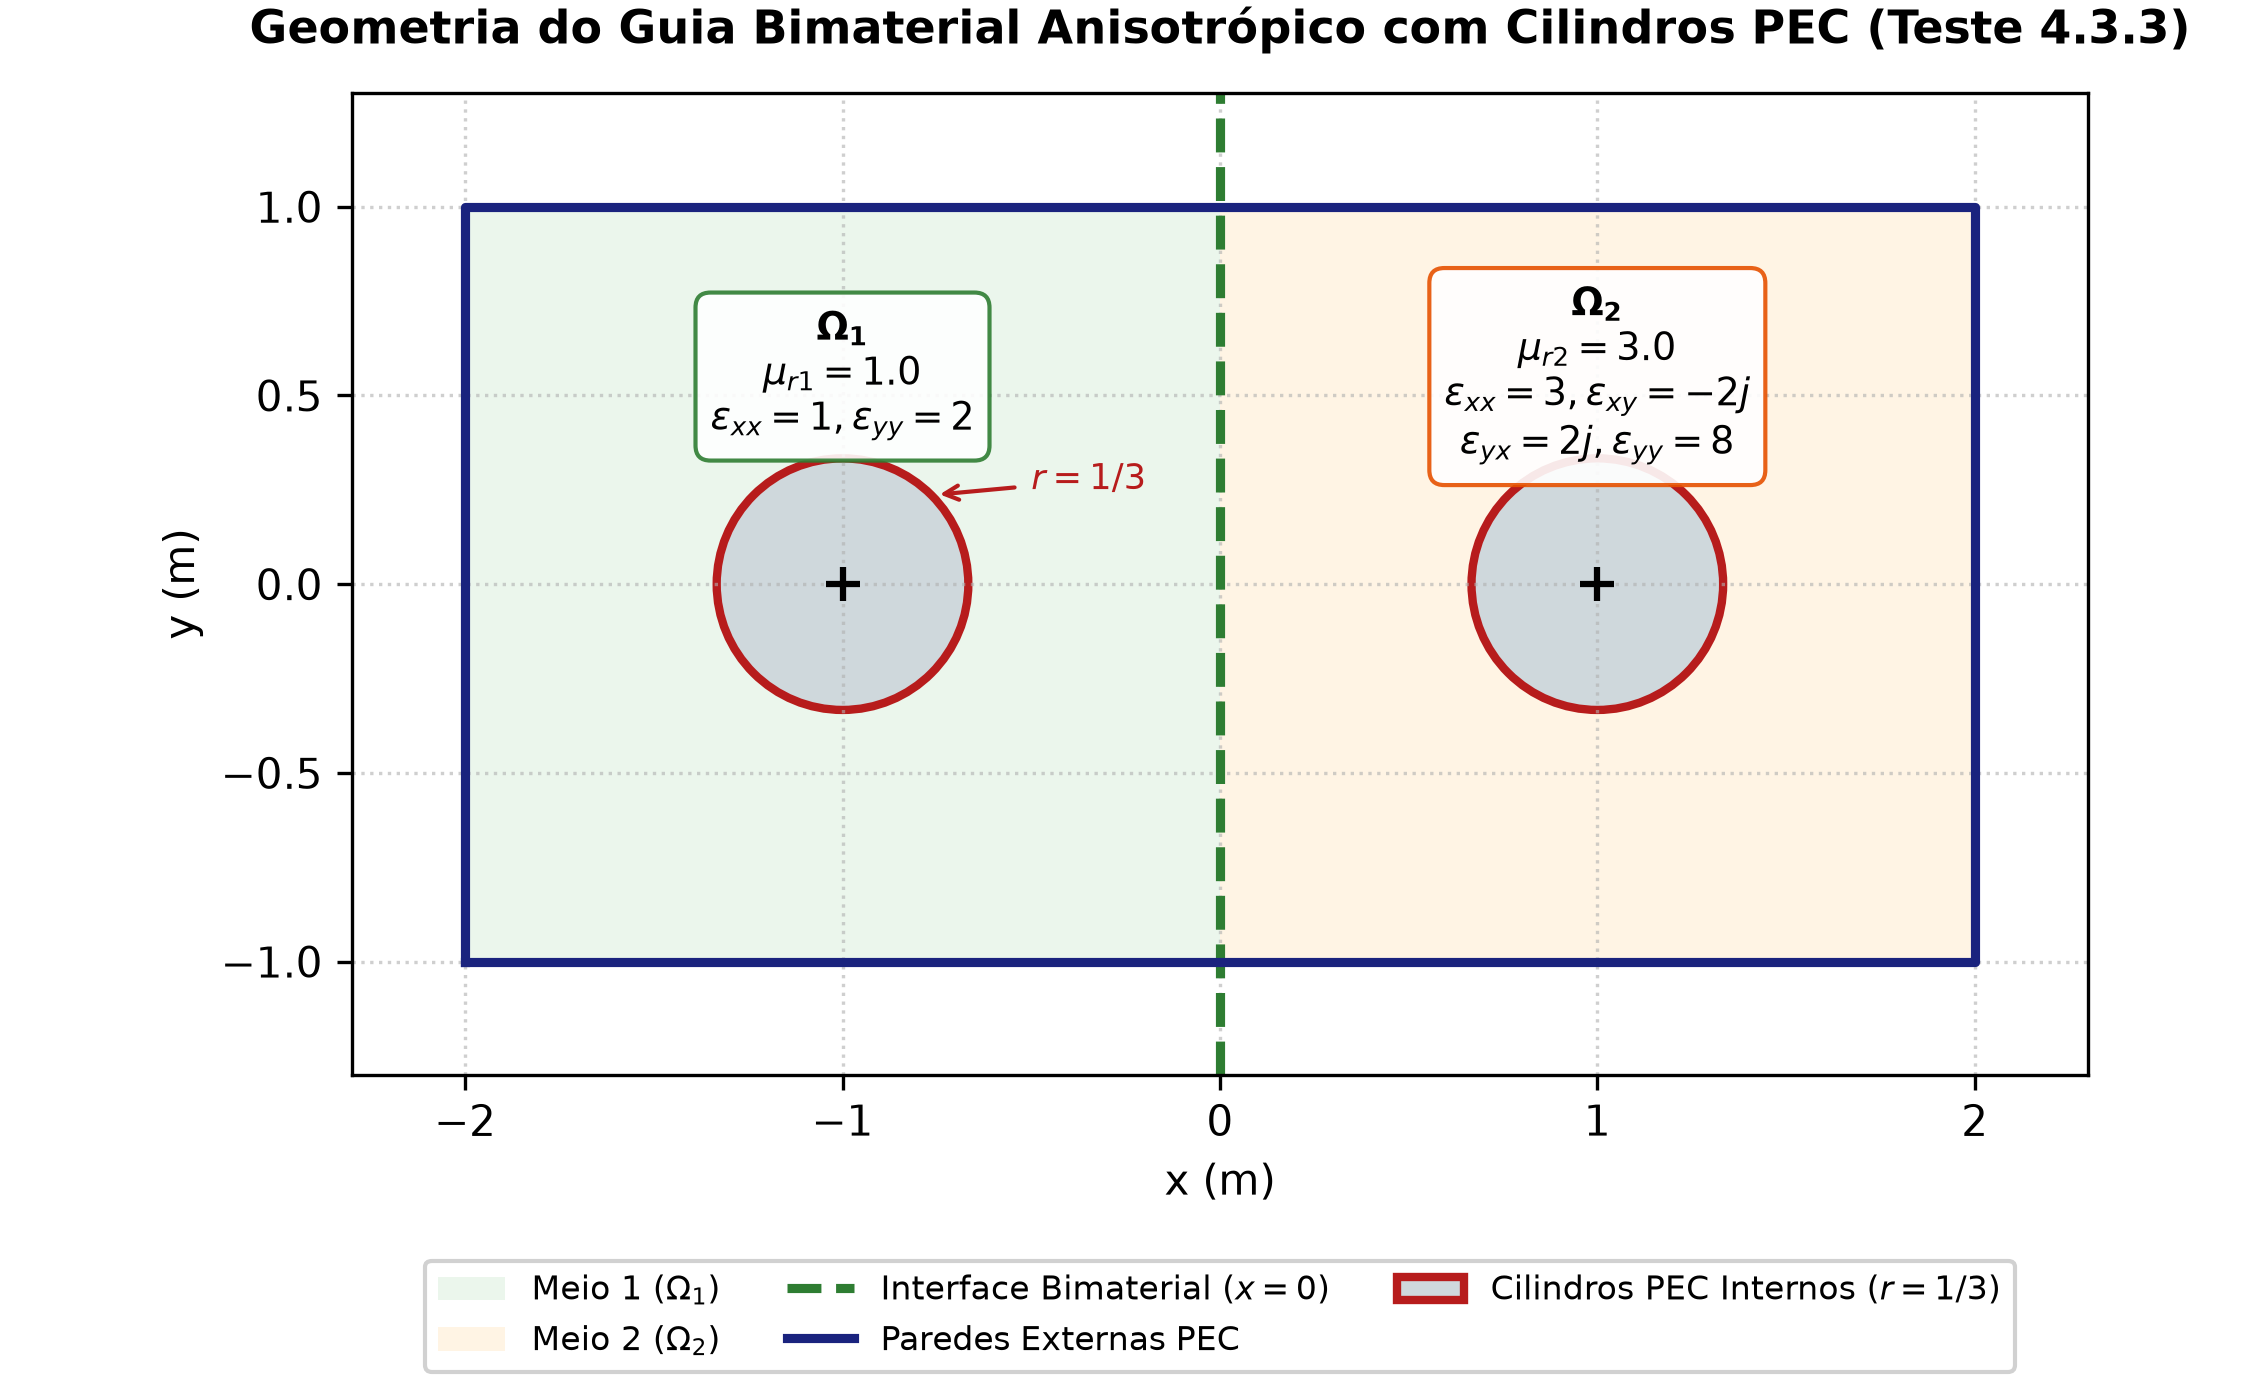
\includegraphics[width=0.85\textwidth]{Geometria_Guia_Bimaterial_Circ.png}
\caption{Geometria do guia bimaterial anisotr\'opico com inclus\~oes cil\'indricas PEC e interface plana em $x = 0$ (Teste 4.3.3).}
\label{fig:geom_circ}
\end{figure}

\begin{table}[H]
\centering
\caption{Compara\c{c}\~ao dos primeiros 5 autovalores no guia bimaterial com inclus\~oes PEC entre o VNMM 2D e o FEM de refer\^encia (340.363 arestas).}
\label{tab:circguide}
\resizebox{\textwidth}{!}{
\begin{tabular}{cccccc}
\toprule
Modo & Ref. FEM (340k arestas) & FEM Misto \cite{jiang2014} & EMM \cite{lima2017} (8.566 ares) & VNMM 2D (Nuvem Nodal) & Erro Relativo (\%) \\
\midrule
\textbf{1} & $0.051876$ & $0.051841$ & $0.051825$ & $0.051641$ & $\mathbf{0.45\%}$ \\
\textbf{2} & $0.205316$ & $0.205012$ & $0.204686$ & $0.203056$ & $\mathbf{1.10\%}$ \\
\textbf{3} & $0.247201$ & $0.247126$ & $0.246919$ & $0.255165$ & $\mathbf{3.22\%}$ \\
\textbf{4} & $0.423569$ & --- & $0.423277$ & $0.414830$ & $\mathbf{2.06\%}$ \\
\textbf{5} & $0.625603$ & --- & $0.624568$ & $0.637011$ & $\mathbf{1.82\%}$ \\
\bottomrule
\end{tabular}}
\end{table}

Mesmo com a complexidade combinada de fronteiras curvas PEC internas, interfaces materiais em $x = 0$ e tensores complexos, o VNMM obteve erro no modo dominante de apenas $\mathbf{0.45\%}$ e erro inferior a $3.3\%$ em todos os modos, comprovando a robustez da formula\c{c}\~ao nodal.

\subsection{Cavidade com Jun\c{c}\~ao Qu\'adrupla de Quatro Materiais (\textit{Quad-Junction})}
Para avaliar o comportamento do m\'etodo diante de uma singularidade cl\'assica de m\'ultiplas interfaces ortogonais se encontrando em um \'unico v\'ertice (teste de estresse para formula\c{c}\~oes sem malha), analisou-se uma cavidade quadrada PEC $\Omega = [-1, 1] \times [-1, 1]\text{ m}$ dividida em quatro quadrantes com permissividades distintas ($\mu_r = 1.0$ em todo o dom\'inio), encontrando-se no ponto central $(0, 0)$:
\begin{itemize}
  \item $Q_1$ ($x < 0, y > 0$): $\varepsilon_{r1} = 1.0$;
  \item $Q_2$ ($x > 0, y > 0$): $\varepsilon_{r2} = 4.0$;
  \item $Q_3$ ($x < 0, y < 0$): $\varepsilon_{r3} = 2.0$;
  \item $Q_4$ ($x > 0, y < 0$): $\varepsilon_{r4} = 9.0$ (contraste m\'aximo $9:1$ no v\'ertice central).
\end{itemize}

Na nuvem de pontos ($624$ n\'os totais: $528$ ativos e $96$ n\'os PEC escalonados, com quadratura de Gauss $3\times 3$ e penalidade $s_{\mathrm{div}} = 10.0$), os n\'os das quatro semi-interfaces ($x = 0$ e $y = 0$) recebem diretores estritamente tangenciais ($\hat{x}$ ou $\hat{y}$), mantendo-se alinhados com os n\'os internos e omitindo-se um n\'o exatamente sobre o ponto de jun\c{c}\~ao qu\'adrupla $(0, 0)$ para evitar super-restri\c{c}\~ao angular. Cada quadrante seleciona seus est\^enceis apenas entre seus pr\'oprios n\'os e os n\'os das duas semi-interfaces adjacentes (Figura~\ref{fig:geom_quad}).

\begin{figure}[H]
\centering
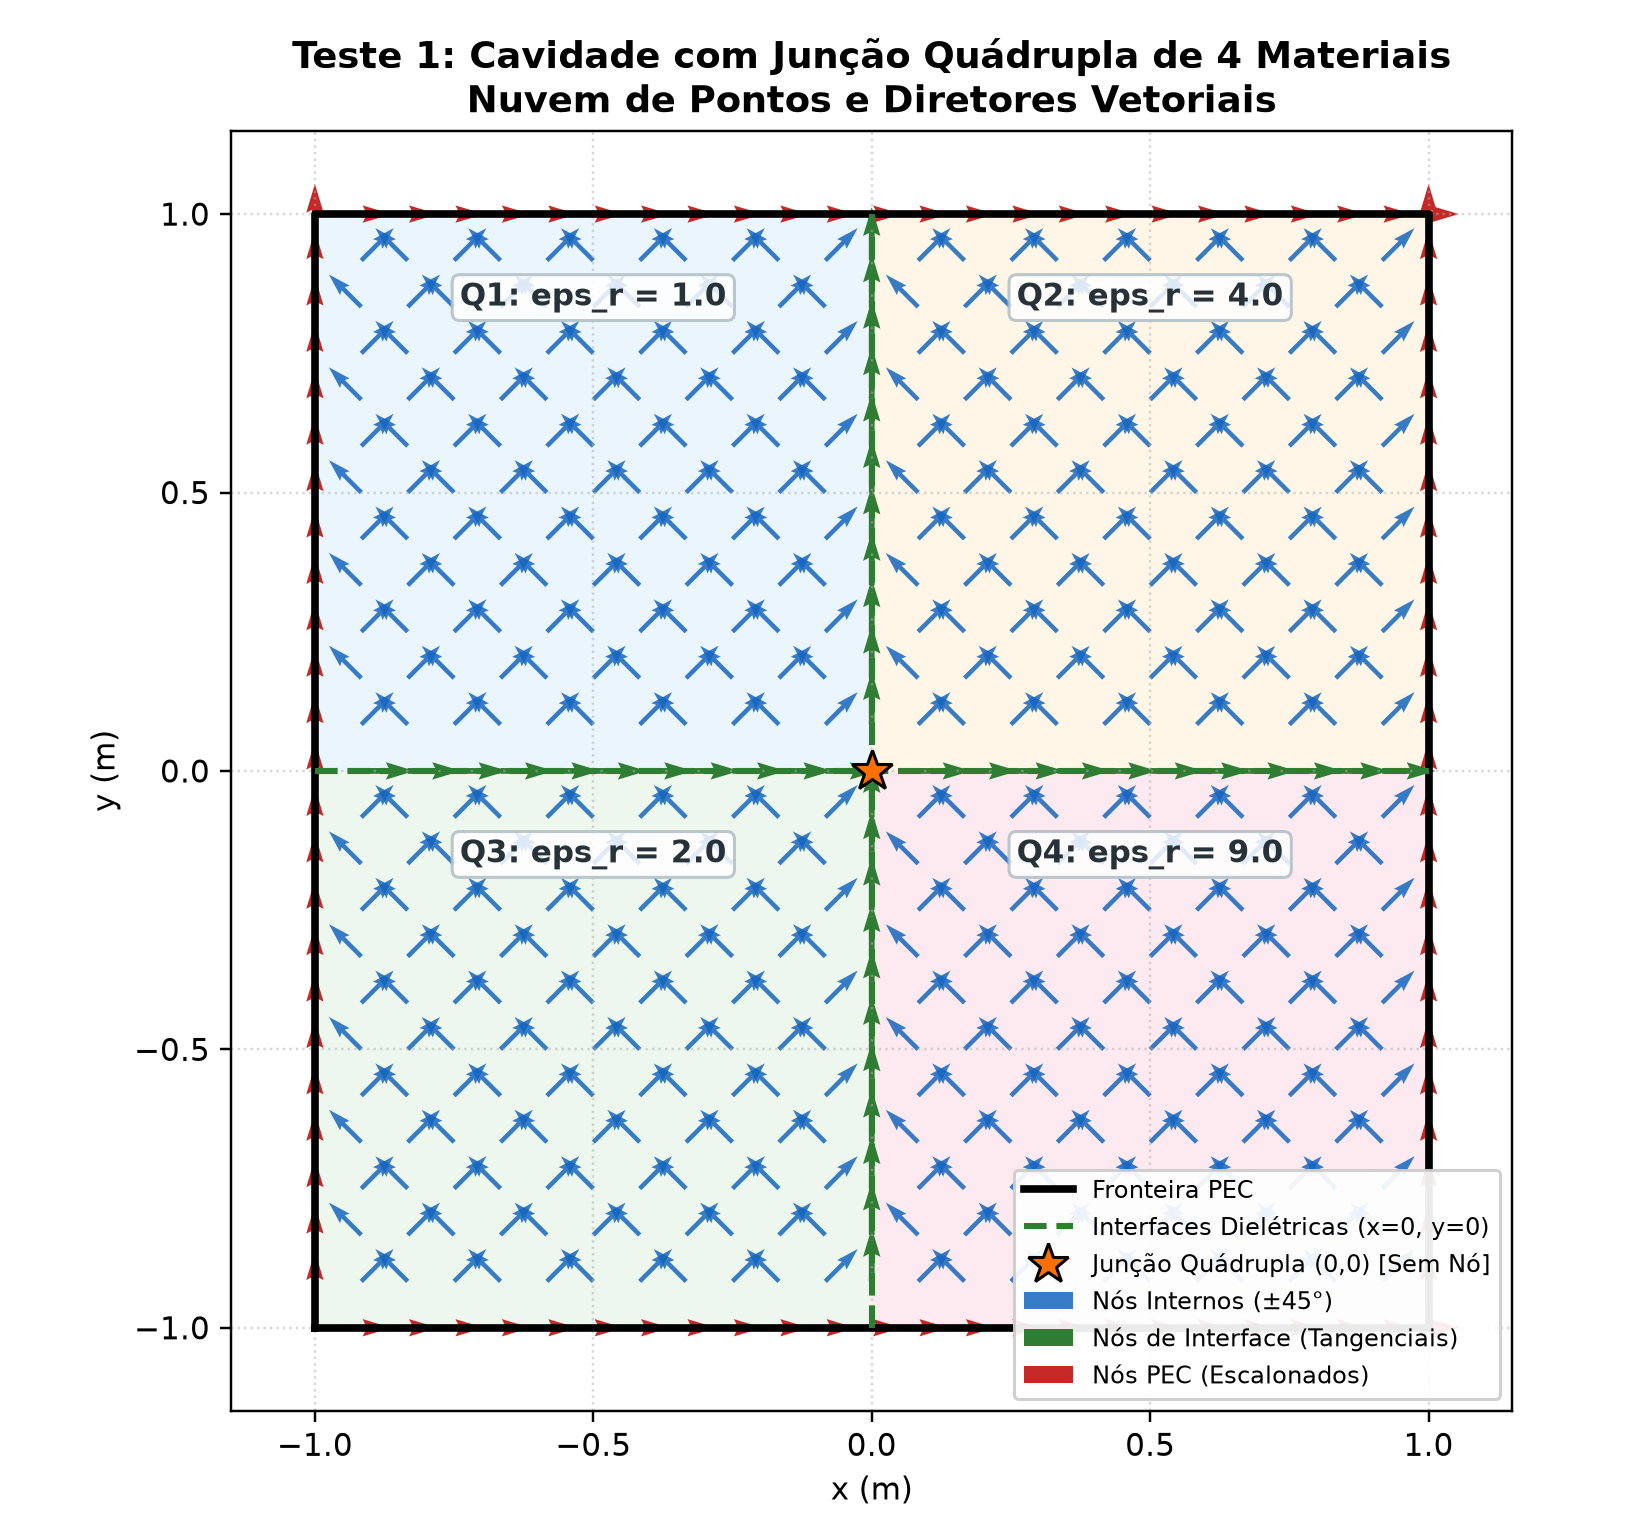
\includegraphics[width=0.72\textwidth]{Geometria_Nuvem_Quad_Junction.png}
\caption{Cavidade com jun\c{c}\~ao qu\'adrupla de 4 materiais distintos encontrando-se em $(0,0)$, ilustrando a nuvem de pontos e a atribui\c{c}\~ao de diretores tangenciais nas 4 semi-interfaces.}
\label{fig:geom_quad}
\end{figure}

Como refer\^encia independente de alta precis\~ao, resolveu-se a formula\c{c}\~ao escalar exata em $H_z$ via Elementos Finitos ($Q_1$) em malha refinada $100 \times 100$ ($10.201$ n\'os), naturalmente livre de modos esp\'urios.

\begin{table}[H]
\centering
\caption{Compara\c{c}\~ao dos primeiros 6 autovalores na cavidade com jun\c{c}\~ao qu\'adrupla (4 materiais) entre o VNMM 2D e o FEM $H_z$ ($100\times 100$).}
\label{tab:quad}
\begin{tabular}{ccccc}
\toprule
Modo & Ref. FEM ($H_z$, $100\times 100$) & VNMM 2D (Nuvem Nodal) & Erro Relativo (\%) & $R_{\mathrm{div}}$ (\%) \\
\midrule
\textbf{1} & $0.515505$ & $0.513771$ & $\mathbf{0.34\%}$ & $0.54\%$ \\
\textbf{2} & $0.747157$ & $0.690568$ & $7.57\%$ & $0.71\%$ \\
\textbf{3} & $1.718475$ & $1.734055$ & $\mathbf{0.91\%}$ & $0.36\%$ \\
\textbf{4} & $2.026521$ & $2.003816$ & $\mathbf{1.12\%}$ & $1.22\%$ \\
\textbf{5} & $2.554525$ & $2.474523$ & $\mathbf{3.13\%}$ & $1.75\%$ \\
\textbf{6} & $3.788495$ & $3.922816$ & $\mathbf{3.55\%}$ & $1.64\%$ \\
\bottomrule
\end{tabular}
\end{table}

\begin{figure}[H]
\centering
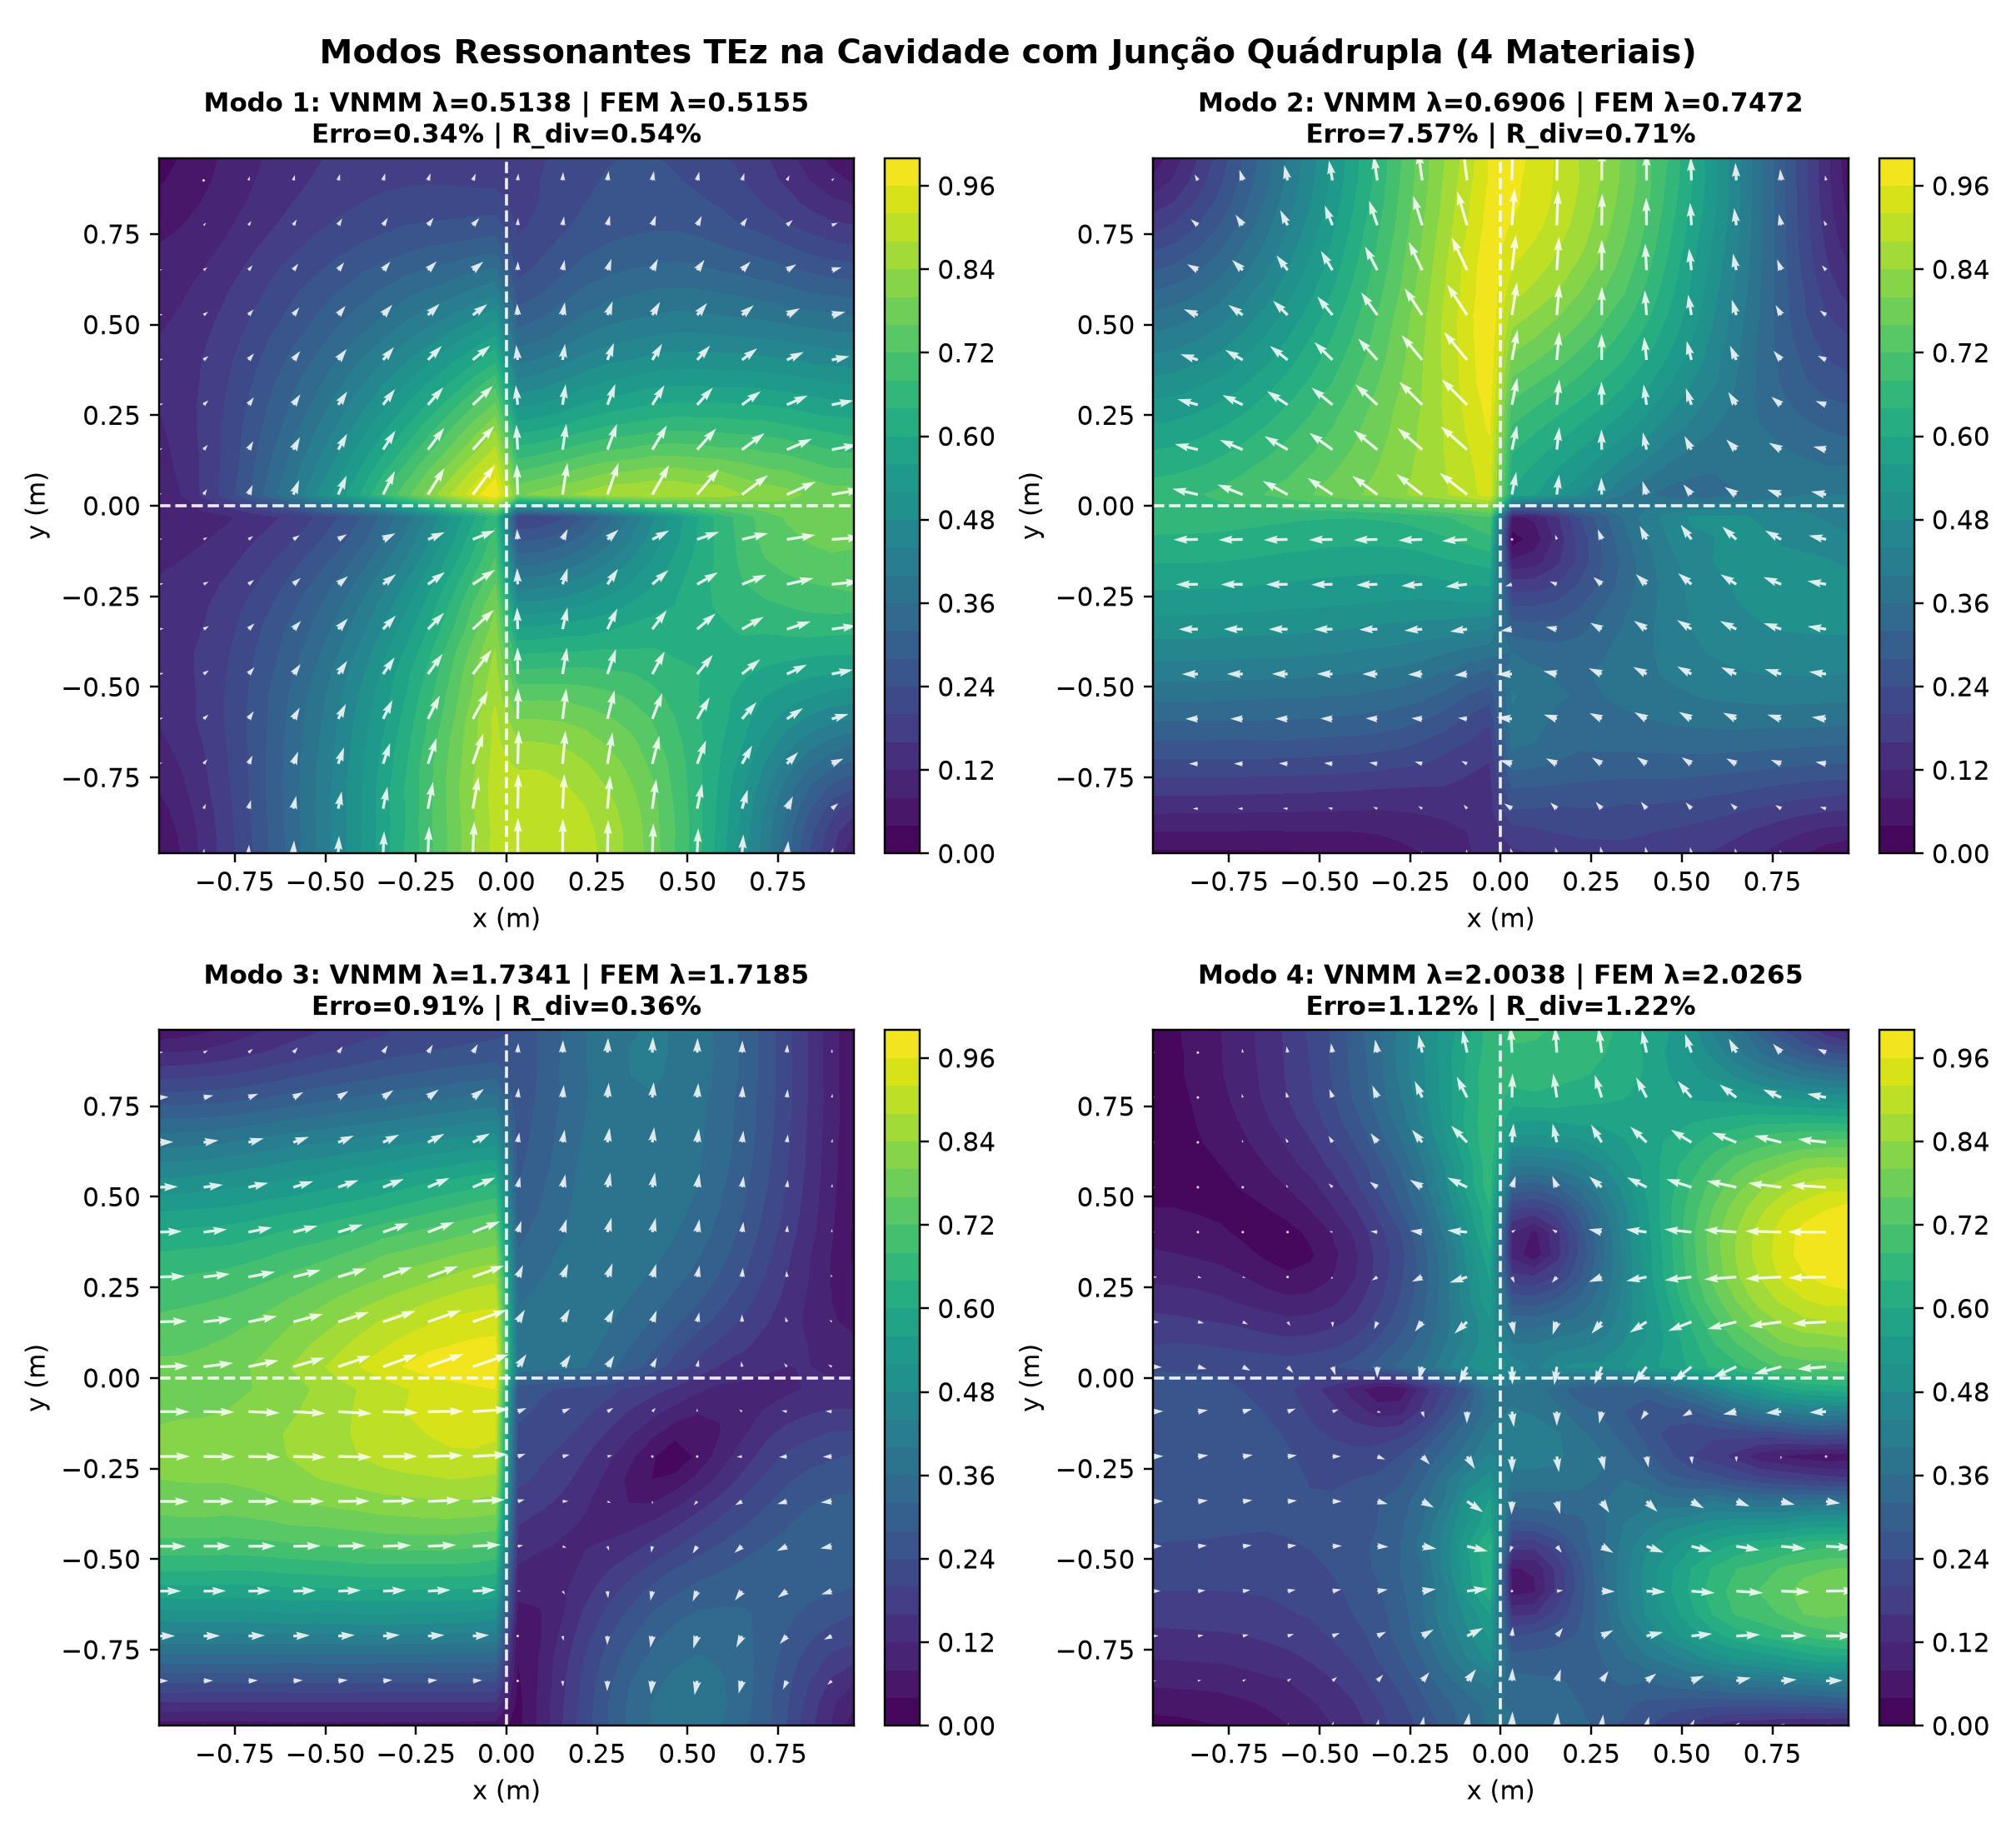
\includegraphics[width=0.90\textwidth]{VNMM_Quad_Junction_Modes.png}
\caption{Distribui\c{c}\~ao espacial de $|\mathbf{E}|$ e vetores de campo dos 4 primeiros modos $\mathrm{TE}_z$ na cavidade com jun\c{c}\~ao qu\'adrupla, evidenciando o salto n\'itido das componentes normais nas interfaces ortogonais e a aus\^encia de modos esp\'urios ($R_{\mathrm{div}} \le 1.22\%$).}
\label{fig:modes_quad}
\end{figure}

Os resultados demonstram que o VNMM captura com precis\~ao a f\'isica singular do encontro de quatro materiais: o modo fundamental apresenta erro de apenas $\mathbf{0.34\%}$, os modos 3 e 4 atingem erros em torno de $\mathbf{1\%}$ e todos os modos exibem baixa energia de diverg\^encia ($R_{\mathrm{div}} < 1.8\%$), comprovando que a arquitetura de parti\c{c}\~ao de suportes e diretores tangenciais se estende naturalmente para v\'ertices de m\'ultiplos materiais.

\section{Conclus\~oes}

O desenvolvimento e a valida\c{c}\~ao do \textbf{Vector Nodal Meshless Method (VNMM 2D)} sobre nuvens de pontos confirmam seu potencial para resolver problemas eletromagn\'eticos avan\c{c}ados:
\begin{enumerate}
  \item \textbf{Completude Reprodutiva e Invari\^ancia Nodal:} A formula\c{c}\~ao baseada em proje\c{c}\~oes direcionais preserva consist\^encia polinomial de primeira ordem em precis\~ao de m\'aquina ($10^{-16}$) independentemente da irregularidade geom\'etrica dos pontos (de 0\% a 50\% de perturba\c{c}\~ao estoc\'astica);
  \item \textbf{Superioridade de Nuvens Irregulares:} A quebra de alinhamentos cartesianos regulares via perturba\c{c}\~ao estoc\'astica atenua o vi\'es direcional da discretiza\c{c}\~ao (\textit{grid-locking}), reduzindo o erro m\'edio dos autovalores em mais de 50\% (para $\approx 1.1\%$) em rela\c{c}\~ao a arranjos regulares r\'igidos;
  \item \textbf{Resolu\c{c}\~ao de Descontinuidades e Jun\c{c}\~oes M\'ultiplas Sem Borramento:} A segrega\c{c}\~ao estrita de suportes por material captura o salto de descontinuidade normal de forma n\'itida, preservando a continuidade tangencial sem oscila\c{c}\~oes de Gibbs --- inclusive em jun\c{c}\~oes qu\'adruplas de quatro meios distintos com contraste $9:1$ (erro de $0.34\%$ no modo fundamental);
  \item \textbf{Generalidade F\'isica em Meios Anisotr\'opicos Complexos:} A formula\c{c}\~ao resolveu com alta acur\'acia (erros de $0.45\%$ a $3.2\%$) problemas de autovalores com tensores diel\'etricos hermitianos, geometrias com quinas vivas e inclus\~oes circulares PEC, equiparando-se a modelos de refer\^encia de elementos finitos de aresta com centenas de milhares de graus de liberdade.
\end{enumerate}

\begin{thebibliography}{9}
\bibitem{harrington2001} R. F. Harrington, \textit{Time-Harmonic Electromagnetic Fields}. IEEE Press / Wiley-Interscience, 2001.
\bibitem{collin1991} R. E. Collin, \textit{Field Theory of Guided Waves}. IEEE Press, 1991.
\bibitem{jin2014} J. M. Jin, \textit{The Finite Element Method in Electromagnetics}. John Wiley \& Sons, 2014.
\bibitem{belytschko1994} T. Belytschko, Y. Y. Lu, and L. Gu, ``Element-free Galerkin methods,'' \textit{Int. J. Numer. Methods Eng.}, vol. 37, no. 2, pp. 229--256, 1994.
\bibitem{ortiz2023} L. A. Garcia Ortiz, \textit{M\'etodo Sem Malha Nodal Utilizando Fun\c{c}\~oes de Forma Vetoriais Baseadas em H(curl)}. Tese de Doutorado, Universidade Federal de Minas Gerais (UFMG), Belo Horizonte, 2023.
\bibitem{ortiz2021} L. A. G. Ortiz, R. C. Mesquita, and N. Z. Lima, ``Nodal meshless method with vectorial shape functions based on H(curl),'' \textit{IEEE Trans. Magn.}, vol. 57, no. 6, pp. 1--4, 2021.
\bibitem{jiang2014} W. Jiang, N. Liu, Y. Tang, and Q. H. Liu, ``Mixed finite element method for 2D vector Maxwell's eigenvalue problem in anisotropic media,'' \textit{Prog. Electromagn. Res.}, vol. 148, pp. 159--170, 2014.
\bibitem{lima2017} N. Z. Lima and R. C. Mesquita, ``Edge meshless method applied to vector electromagnetic problems,'' \textit{IEEE Trans. Magn.}, vol. 53, no. 6, pp. 1--4, 2017.
\end{thebibliography}

\end{document}
